%
% $Id: blank.tex,v 2.0 2010-01-05 18:50:50+09 kobayasi Exp $
%
% Mar 21, 2001:  Revision Control Started!!
%
\documentclass[11pt]{jreport}
\usepackage{newcent}             % PDFへの変換後の品質を高める
\usepackage[dvipdfmx]{graphicx}
\usepackage{color}
\definecolor{purple}{rgb}{0.6,0,0.4}
\definecolor{brown}{cmyk}{0,0.81,1,0.60}
\usepackage{listings, jlisting}
\renewcommand{\lstlistingname}{ソース}
\lstset
{
breaklines = true,
language=Java,
keywordstyle={\color{purple}},
commentstyle={\color{brown}},
numbers=left,
frame=single,
tabsize=4,
}

%\renewcommand{\slash}{"/"}
\renewcommand{\slash}{/}
\graphicspath{{./Screenshots/}, {./Graphs/}} %Where the app screenshots folder is located

%
%\usepackage[doctor]{gaiyo}      % 博士論文要旨の場合
%\usepackage[master]{gaiyo}      % 修士論文要旨の場合
\usepackage{sotsuron}               % 卒業研究概要の場合
% \usepackage[junior]{gaiyo}      % 専門演習レポートの場合

\setlength\textfloatsep{0pt}

\title{\bfseries スマートフォンのモーションセンサを利用した\\個人認証アプリケーションの開発}
\author{情11-170 高坂 賢佑}
\date{}
\renewcommand{\bibname}{参考文献,参考URL等}

\begin{document}
\maketitle

\tableofcontents
\listoffigures

\chapter*{はじめに}
スマートフォンが徐々に普及しつつある現在,スマートフォンの個人認証方法は画面上に表示されるソフトウェアキーボードのテンキーを用いたパスコード認証が大部分を占めている.
しかし,この認証方法は画面ロックを解除するたびに画面に表示されたソフトウェアキーボードを目で見て指でタッチして操作する必要があるため,ユーザにとって煩雑な作業である.
また,あらかじめ決められた文字種の中から一つずつ選択したものを元にパスコードを構築していくという性質上,パターン数が限られ自由度が限定されてしまう.

そこで,パスコード認証が抱える認証の煩雑さを解消し,かつ自由度が高くより直感的に個人認証を行えるアプリケーションを開発する.
このアプリケーションには,一般的なスマートフォンに搭載されている加速度センサとジャイロセンサを用いる.

\chapter{使用するセンサについて}
本アプリケーションには2種類のモーションセンサを利用する.

	\section{加速度センサ}
	加速度センサとは,X軸,Y軸,Z軸の基準軸に対して直線運動の加速度をそれぞれ検出し,値として取り出すことのできるセンサである.
	ここでいう加速度とは,端末における単位時間あたりの速度の変化率のことを指し,図\ref{sensor}における直線で示した矢印の方向が正の値,逆が負の値をとる.
	
	\section{ジャイロセンサ}
	ジャイロセンサとは,X軸,Y軸,Z軸の基準軸に対して回転運動の角速度をそれぞれ検出し,値として取り出すことのできるセンサである.
    ここでいう角速度とは,端末における単位時間あたりの回転角のことを指し,図\ref{sensor}における橙色で示した回転の方向が正の値,逆が負の値をとる.

    % センサのイメージ図
    \begin{figure}[htbp]
      \begin{center}
        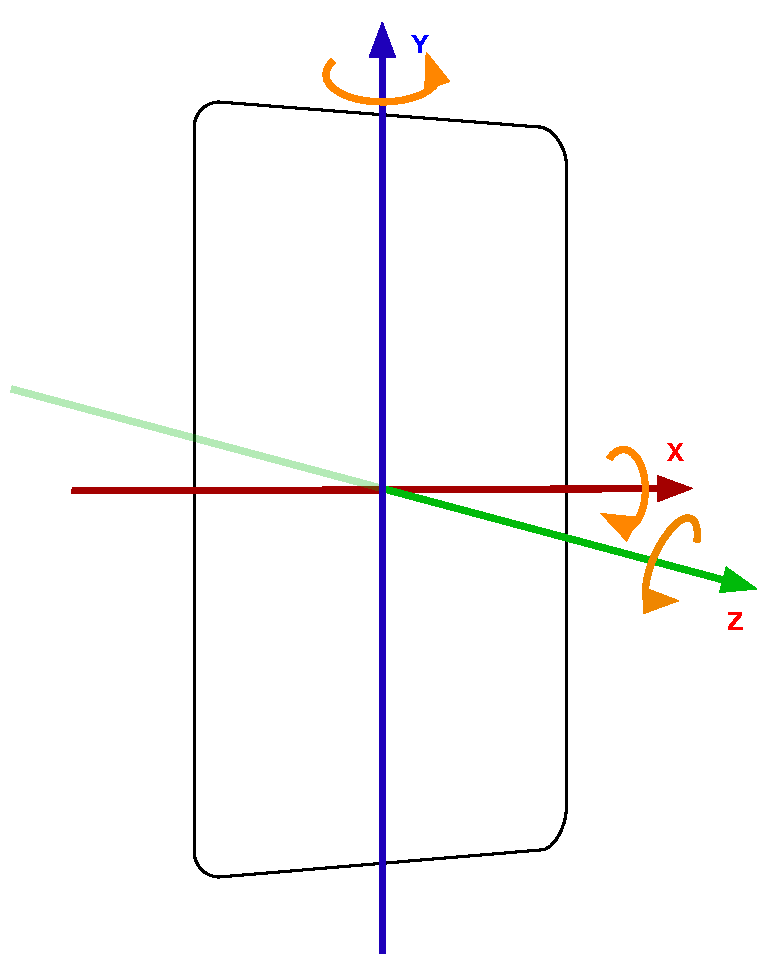
\includegraphics[width=7cm, bb=0 0 373 469]{SmartphoneSensor.pdf}
        \caption{モーションセンサの座標系イメージ}
        \label{sensor}
      \end{center}
    \end{figure}

\chapter{先行研究}
	\section{坂本の研究}
	坂本の研究\cite{sakamoto}では,ユーザが入力したモーションの数値化に加速度センサを用い,あらかじめ保存しておいた複数のジェスチャパターンのデータと認証時に入力したデータをパターンマッチング方式のアルゴリズムを用いて比較することで個人認証を行った.

    しかし,このプログラムは扱うジェスチャによって認証率が高いものと低いものの二分化の傾向が見られるという問題点があった.

	\section{兎澤の研究}
    兎澤の研究\cite{tozawa}では,モーションの数値化に加速度センサとジャイロセンサを用い,認証システムの中核に相関関数を用いたシステムを開発し,ユーザに3回入力させたモーションの平均値データと認証時に入力したデータの類似性を調べることで個人認証を行った.
    これにより,坂本の研究で指摘されていた成功率の二分化や立体的な動きへの対応を可能にし,モーションの対応幅を広げることができた.

    しかし,全体的な認証成功率が低く,特に手首のスナップを用いるような動きの小さいモーションに対して認証率が特に低く出るなど,対応できるモーションに限りがあるという問題点が指摘されていた.

\chapter{本研究のシステム}
	\section{本研究の概要}
	本研究では兎澤の研究で挙げられていた,全体的な認証成功率の低さや対応できるモーションに限りがあるという点を改善することを目標とする.
    具体的には,より幅広いモーション,特に手首のスナップを用いるような比較的動きの小さいモーションに対しての個人認証の全体的な認証成功率の向上を目指し,より実用レベルに近いアプリケーションの開発を行う.

	\section{システムの概要}
	本研究では,先行研究をもとにAndroidデバイス上で動作するアプリケーションとしてシステムを構築する.
    システムの動作フローを図\ref{flow}に示す.

    % システム動作フロー図
    \begin{figure}[hbtp]
        \begin{center}
            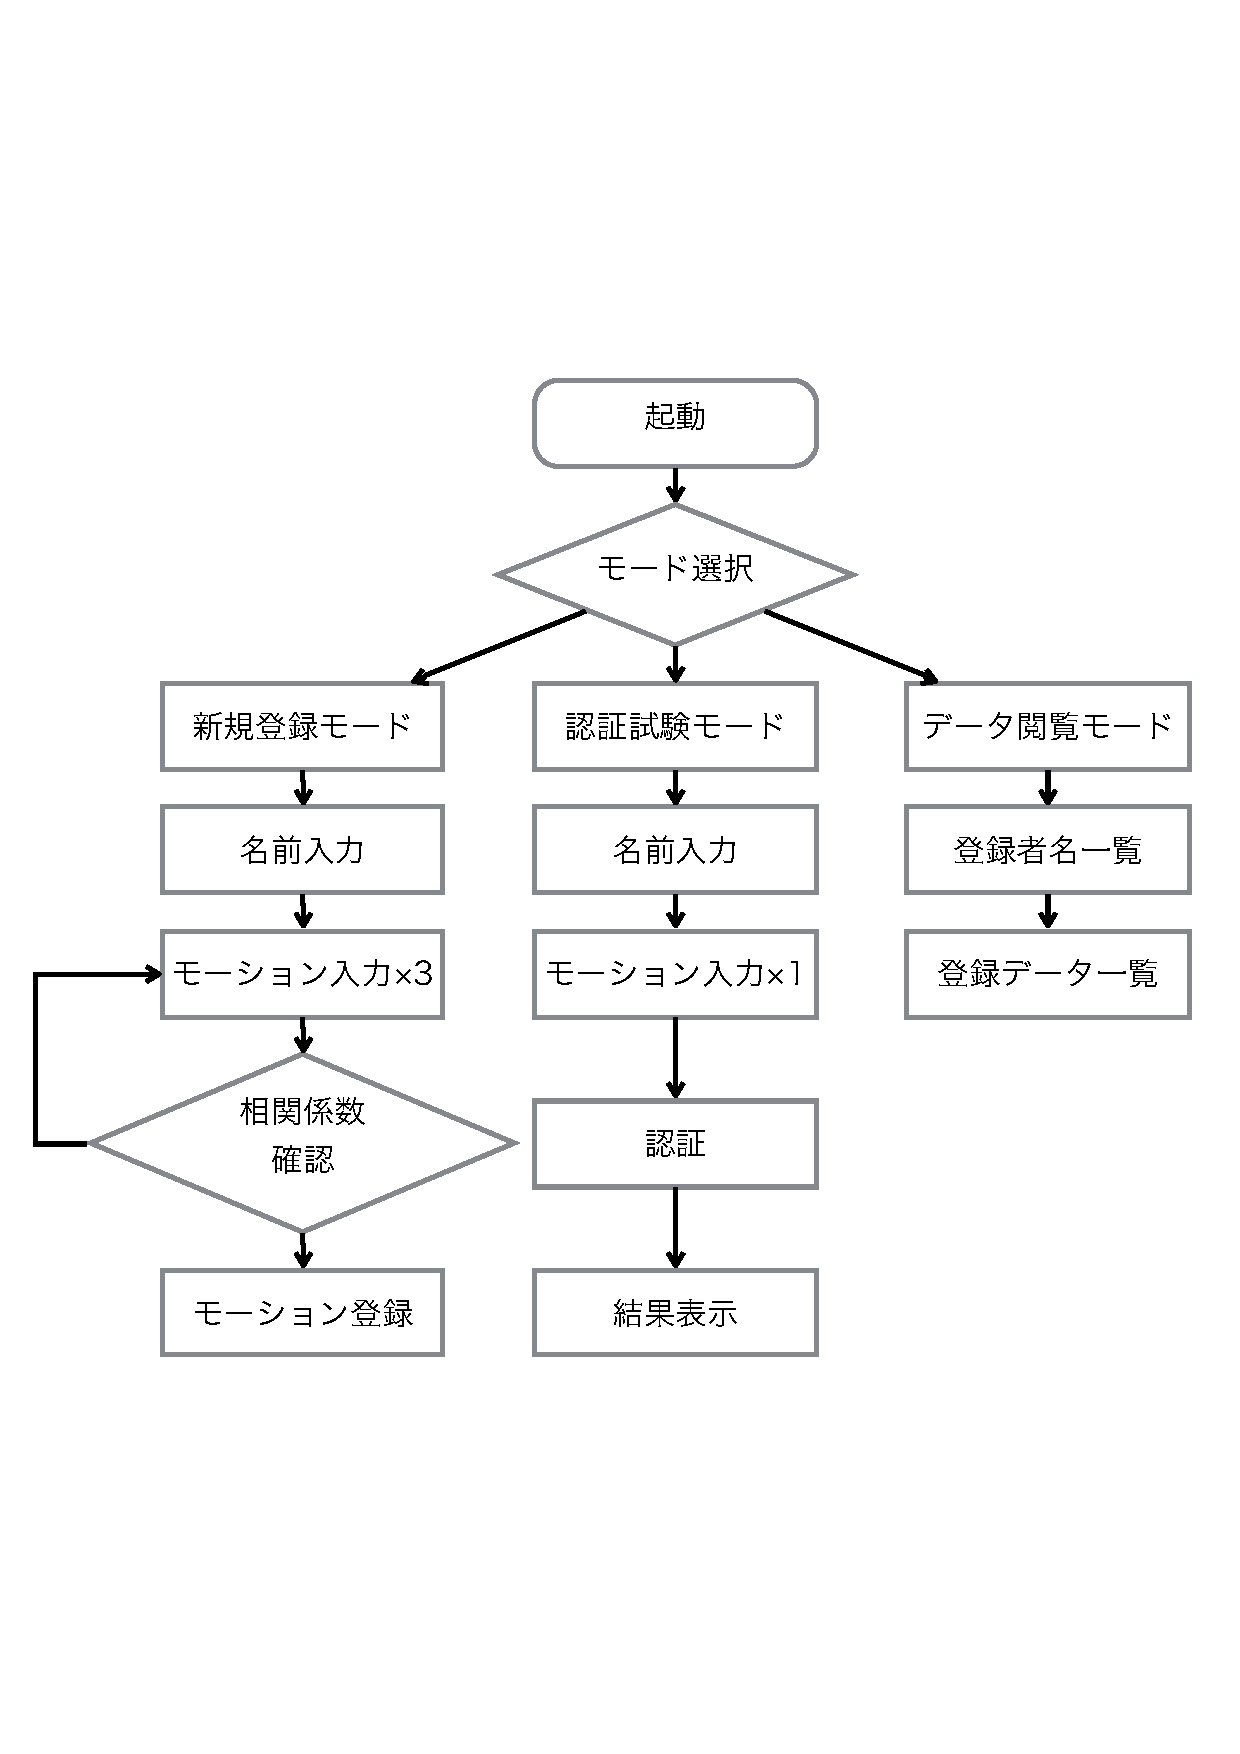
\includegraphics[width=9cm, bb=0 183 594 670]{Flow.pdf}
            \caption{システム動作フロー図}
            \label{flow}
        \end{center}
    \end{figure}

    アプリケーション起動時は,図\ref{start}のような起動画面が表示される.
    ここでStartボタンを押すことで,図\ref{selectMode}のようなモード選択ダイアログが表示される.

    ユーザはまず,新規登録モードにおいて個人認証に用いる鍵情報となるモーションをユーザ名と共に登録する.
    このモードでは,ユーザに同一のモーションを3回入力させ,入力された3回のモーションが同一のモーションであると確認できた場合にそのモーションの平均値をユーザのモーションデータとして登録する.

    認証試験モードでは,事前に新規登録モードにおいてモーションデータを登録しておいたユーザ名を入力させ,該当ユーザが登録されていると確認できた場合にのみ,ユーザにモーションを1回入力させる.
    この入力されたモーションデータと指定したユーザ名で登録されたモーションデータ間の相関を取ることで個人認証を行う.

    データ閲覧モードでは,新規登録モードにおいて登録したユーザ名およびモーションデータをリスト形式で閲覧することが出来る.

    % スタート画面スクリーンショット
    \begin{figure}[htbp]
        \begin{minipage}{0.5\hsize}
            \begin{center}
                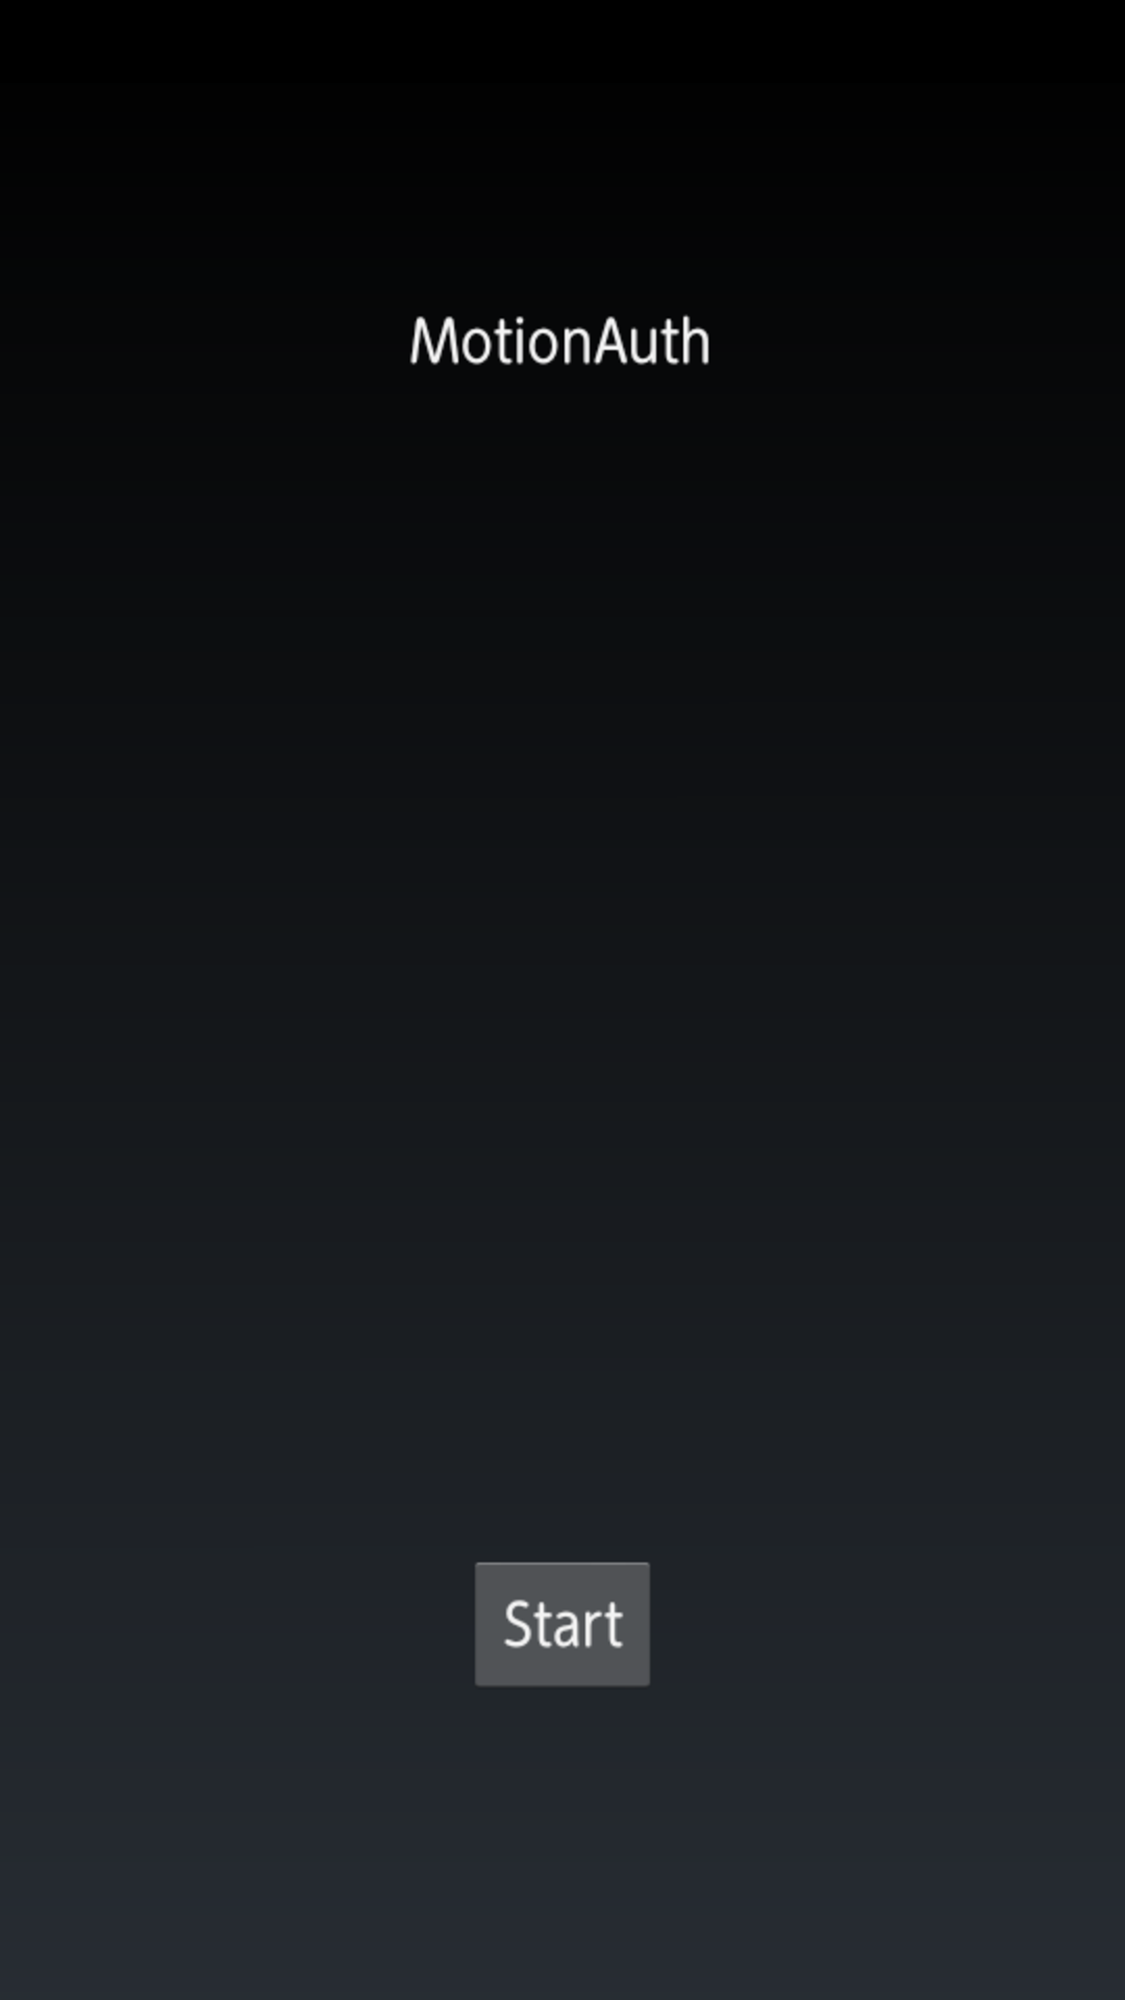
\includegraphics[width=5cm, bb=0 0 540 960]{Start.pdf}
            \end{center}
            \caption{スタート画面}
            \label{start}
        \end{minipage}
        \begin{minipage}{0.5\hsize}
            \begin{center}
                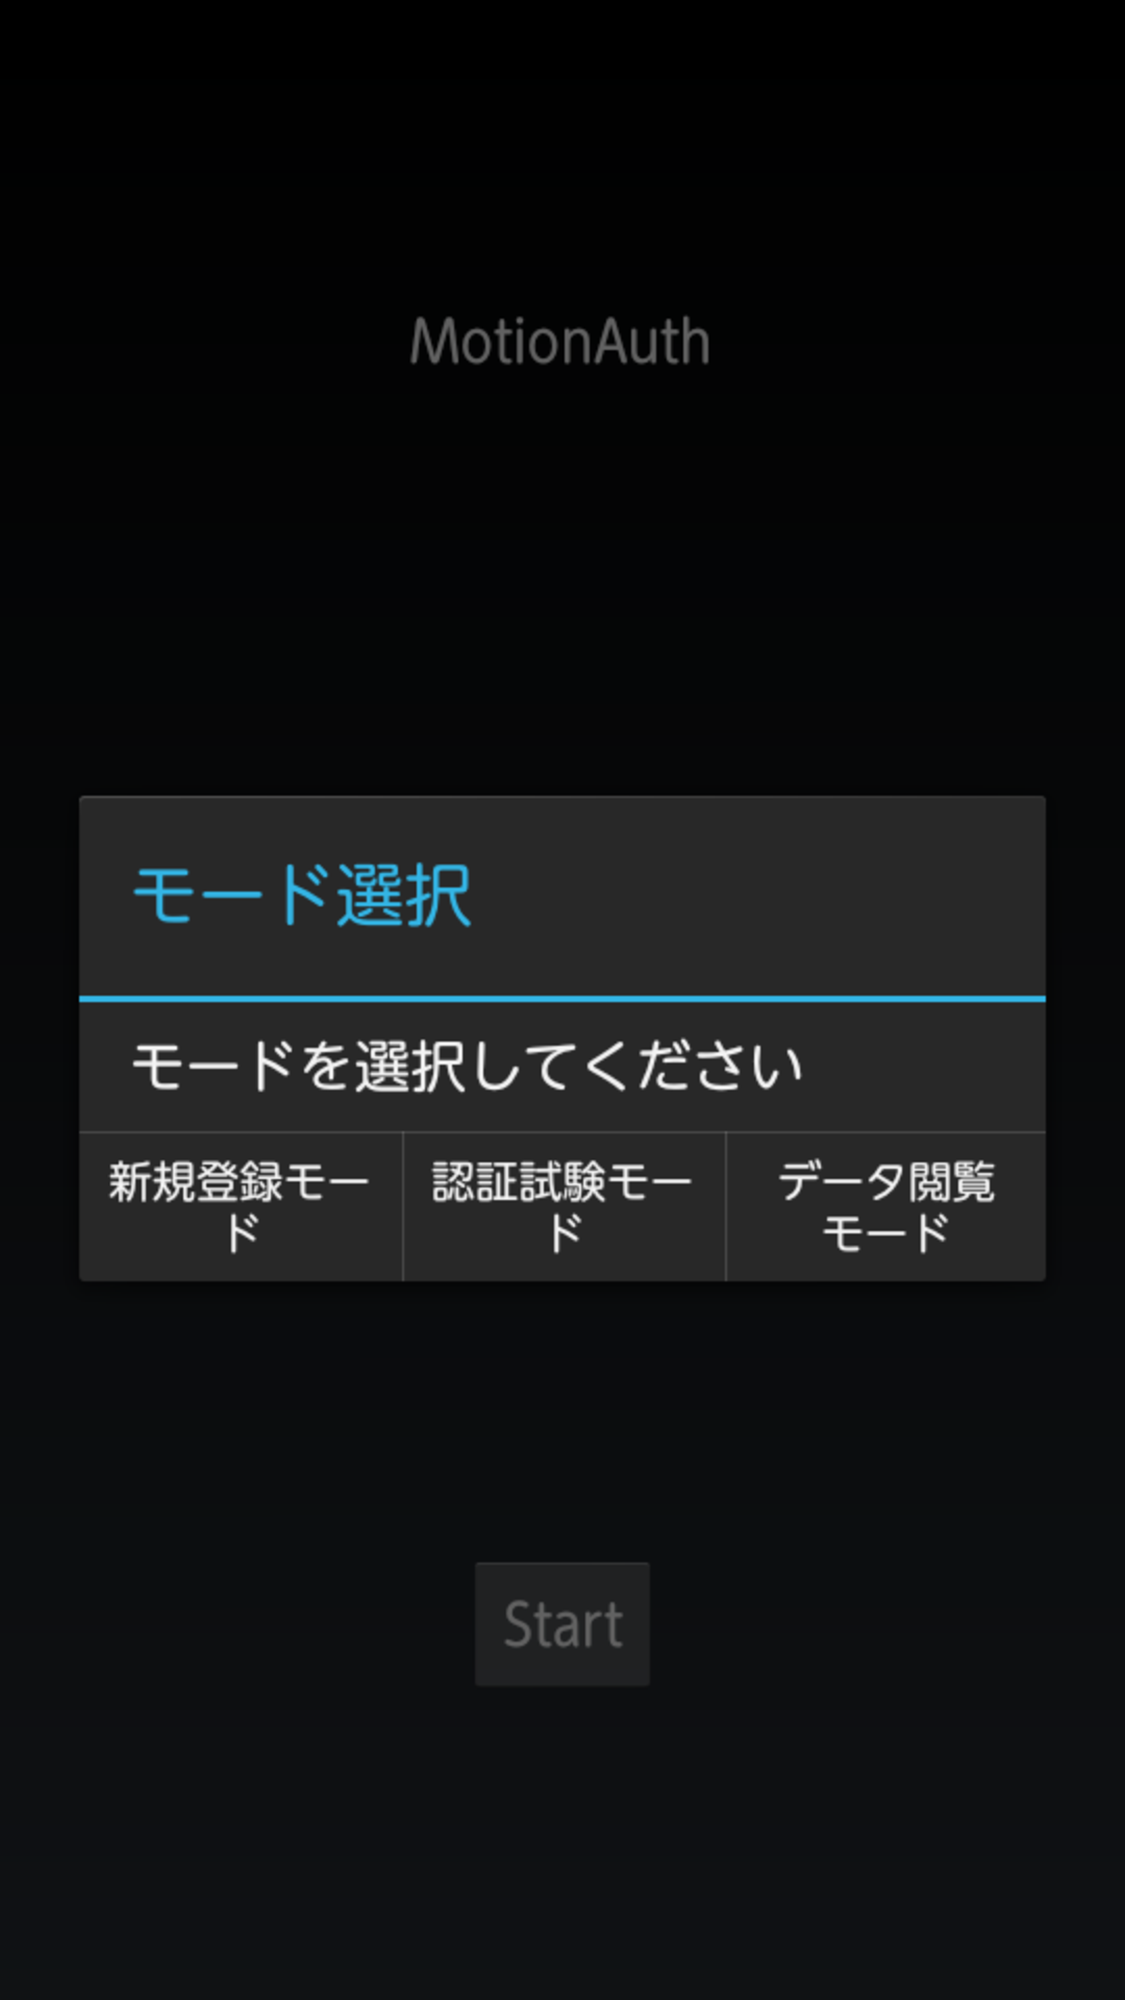
\includegraphics[width=5cm, bb=0 0 540 960]{ModeSelect.pdf}
            \end{center}
            \caption{モード選択ダイアログ}
            \label{selectMode}
        \end{minipage}
    \end{figure}

        % 各モードに対して,説明をもっと掘り下げる
	    \subsection{新規登録モード}
        新規登録モードでは,まず図\ref{nameInput}の画面にて登録したいユーザの名前を入力させる.
        この画面においてOKボタンを押した際にテキストフィールドが空であれば,図\ref{nameInputError}のような通知を表示してユーザに名前の再入力を促す.
        テキストフィールドが空でなければ,次の図\ref{reg}の画面にてモーションの登録を行わせる.
        OKボタンを押した際の名前の入力値チェックを行うコードをソースコード\ref{regCheckInputNameSource}に示す.

        % ユーザ名入力画面
        \begin{figure}[htbp]
            \begin{minipage}{0.33\hsize}
                \begin{center}
                    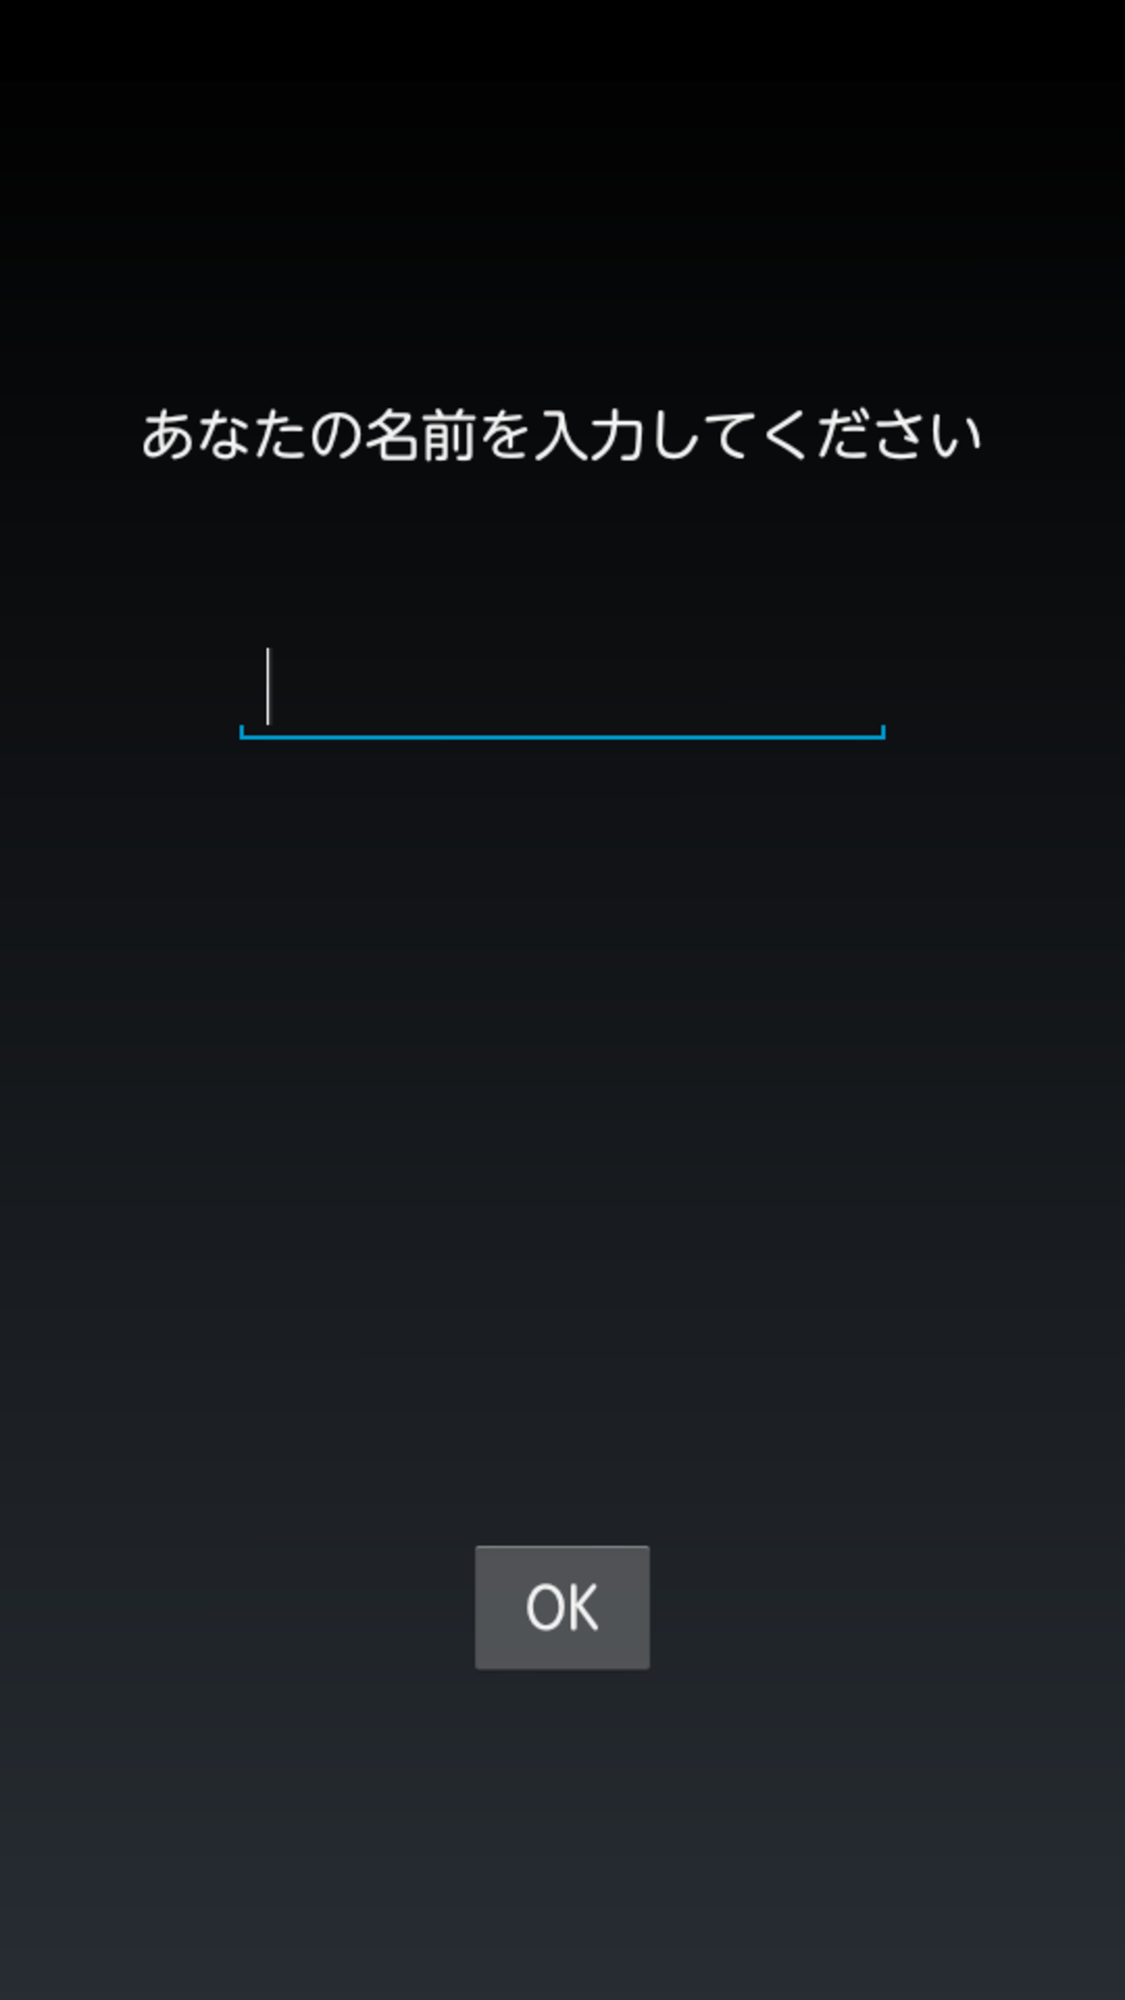
\includegraphics[width=5cm, bb=0 0 540 960]{NameInput.pdf}
                \end{center}
                \caption{ユーザ名入力画面}
                \label{nameInput}
            \end{minipage}
            \begin{minipage}{0.33\hsize}
                \begin{center}
                    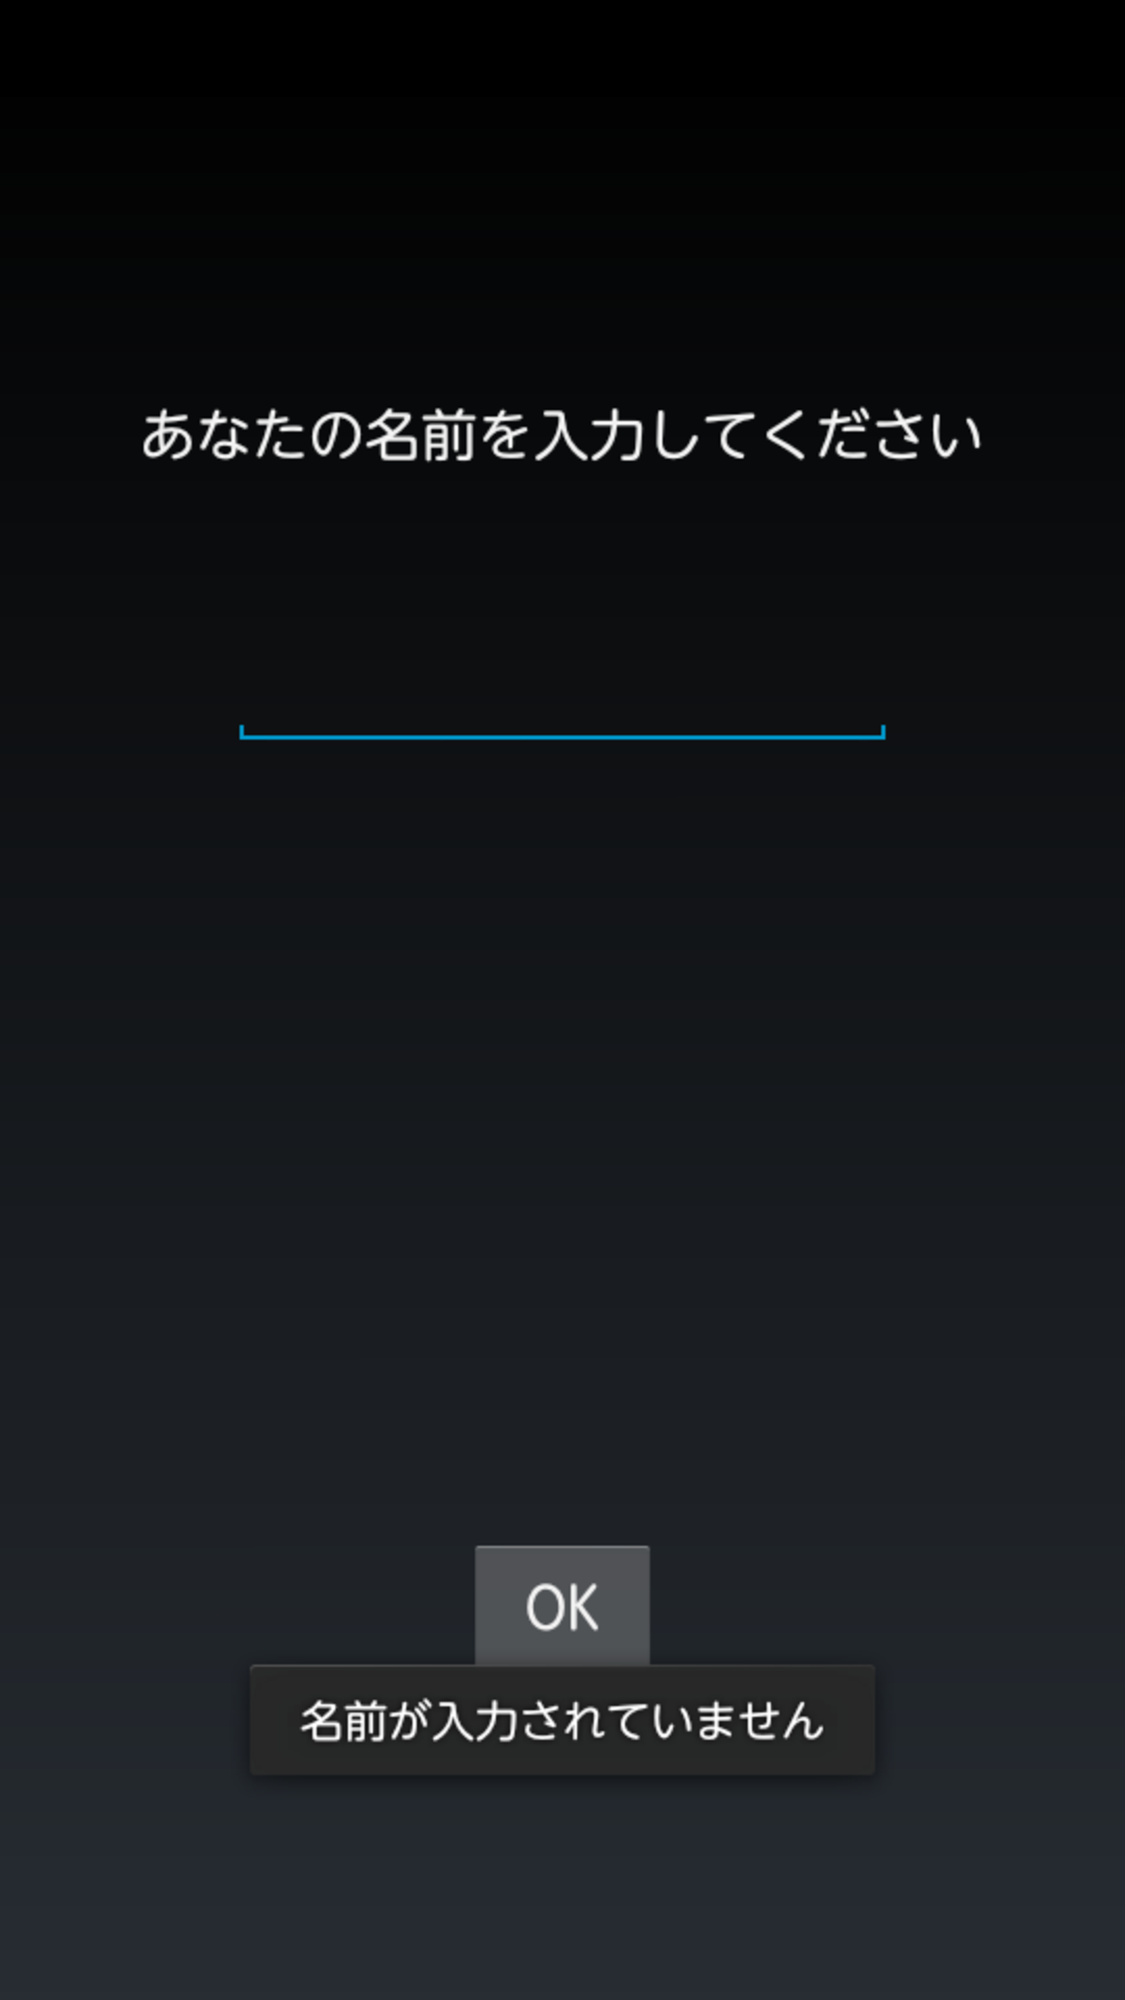
\includegraphics[width=5cm, bb=0 0 540 960]{NameInputError.pdf}
                \end{center}
                \caption{エラー通知}
                \label{nameInputError}
            \end{minipage}
            \begin{minipage}{0.33\hsize}
                \begin{center}
                    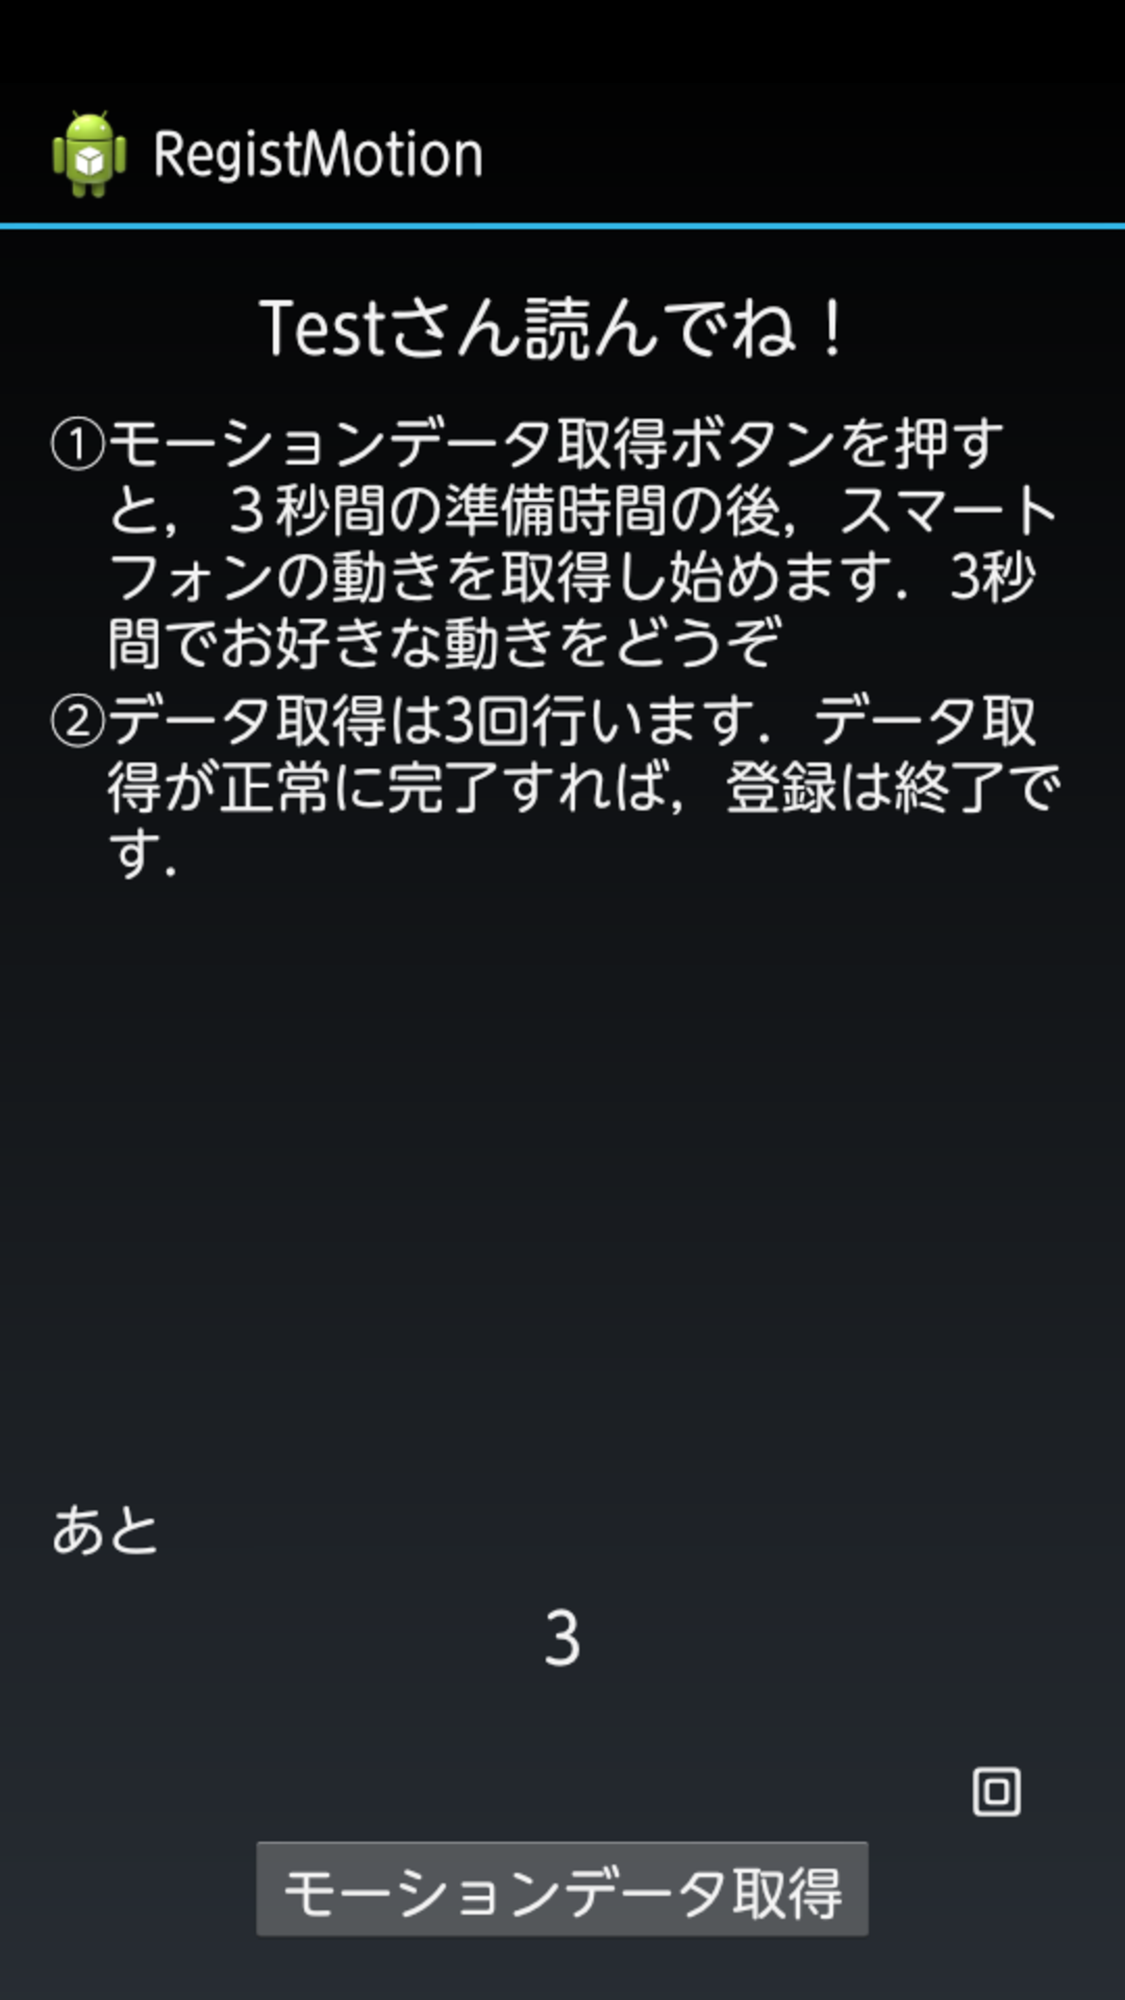
\includegraphics[width=5cm, bb=0 0 540 960]{Reg.pdf}
                \end{center}
                \caption{モーション登録画面}
                \label{reg}
            \end{minipage}
        \end{figure}

        \newpage

        \lstinputlisting[caption=入力値チェック, label=regCheckInputNameSource]
        {Code\slash regCheckInputName}
    
        モーション登録画面においてモーションデータ取得ボタンを押すと,3秒間のインターバルを挟んだ後にモーションデータの取得を3秒間行う.
        この際,画面の下部にそれぞれの経過秒数を表示し,ヴァイブレーションにて1秒毎の時間経過を知らせるようにしている.

        モーションデータの取得は加速度データ,ジャイロデータそれぞれを0.03秒ごとにセンサから取得し,X・Y・Z軸のそれぞれから100個ずつ,計600個を1回分として取得する.

        モーションデータの取得が3回行われると図\ref{regProgress}のような計算処理待ちダイアログが表示され,データの加工が行われる.
        あらかじめ増幅器の閾値と増幅量を設定しておき,取得したデータの振れ幅が閾値よりも小さい場合はモーションの動きが小さいと判断してデータの増幅処理を行う.
        次にモーション取得時の手の細かなブレなどから生じうるデータに対する影響を取り除く,フーリエ変換を用いたローパスフィルタ処理を行う.
        ローパスフィルタ処理が終われば,取得した回数ごとのデータが同一のものであるかの確認を行い,確認されればモーション取得時に生じうる時間的なズレを必要に応じて修正する.
        ズレ修正の処理が終われば3回分のデータ間の相関係数を算出し,相関が認められた場合は図\ref{regSuccess}のような登録完了ダイアログを表示する.
        このダイアログのOKボタンを押すことで,取得した3回分のデータの平均値データを保存し,起動画面に移動する.
        相関が認められなかった場合は,図\ref{regFail}のような登録失敗ダイアログを表示する.
        このダイアログのOKボタンを押すことでプログラム内部のモーションデータ取得カウンタが初期化され,モーションデータの取り直しをさせる.

        % モーション登録画面
        \begin{figure}[htbp]
            \begin{minipage}{0.33\hsize}
                \begin{center}
                    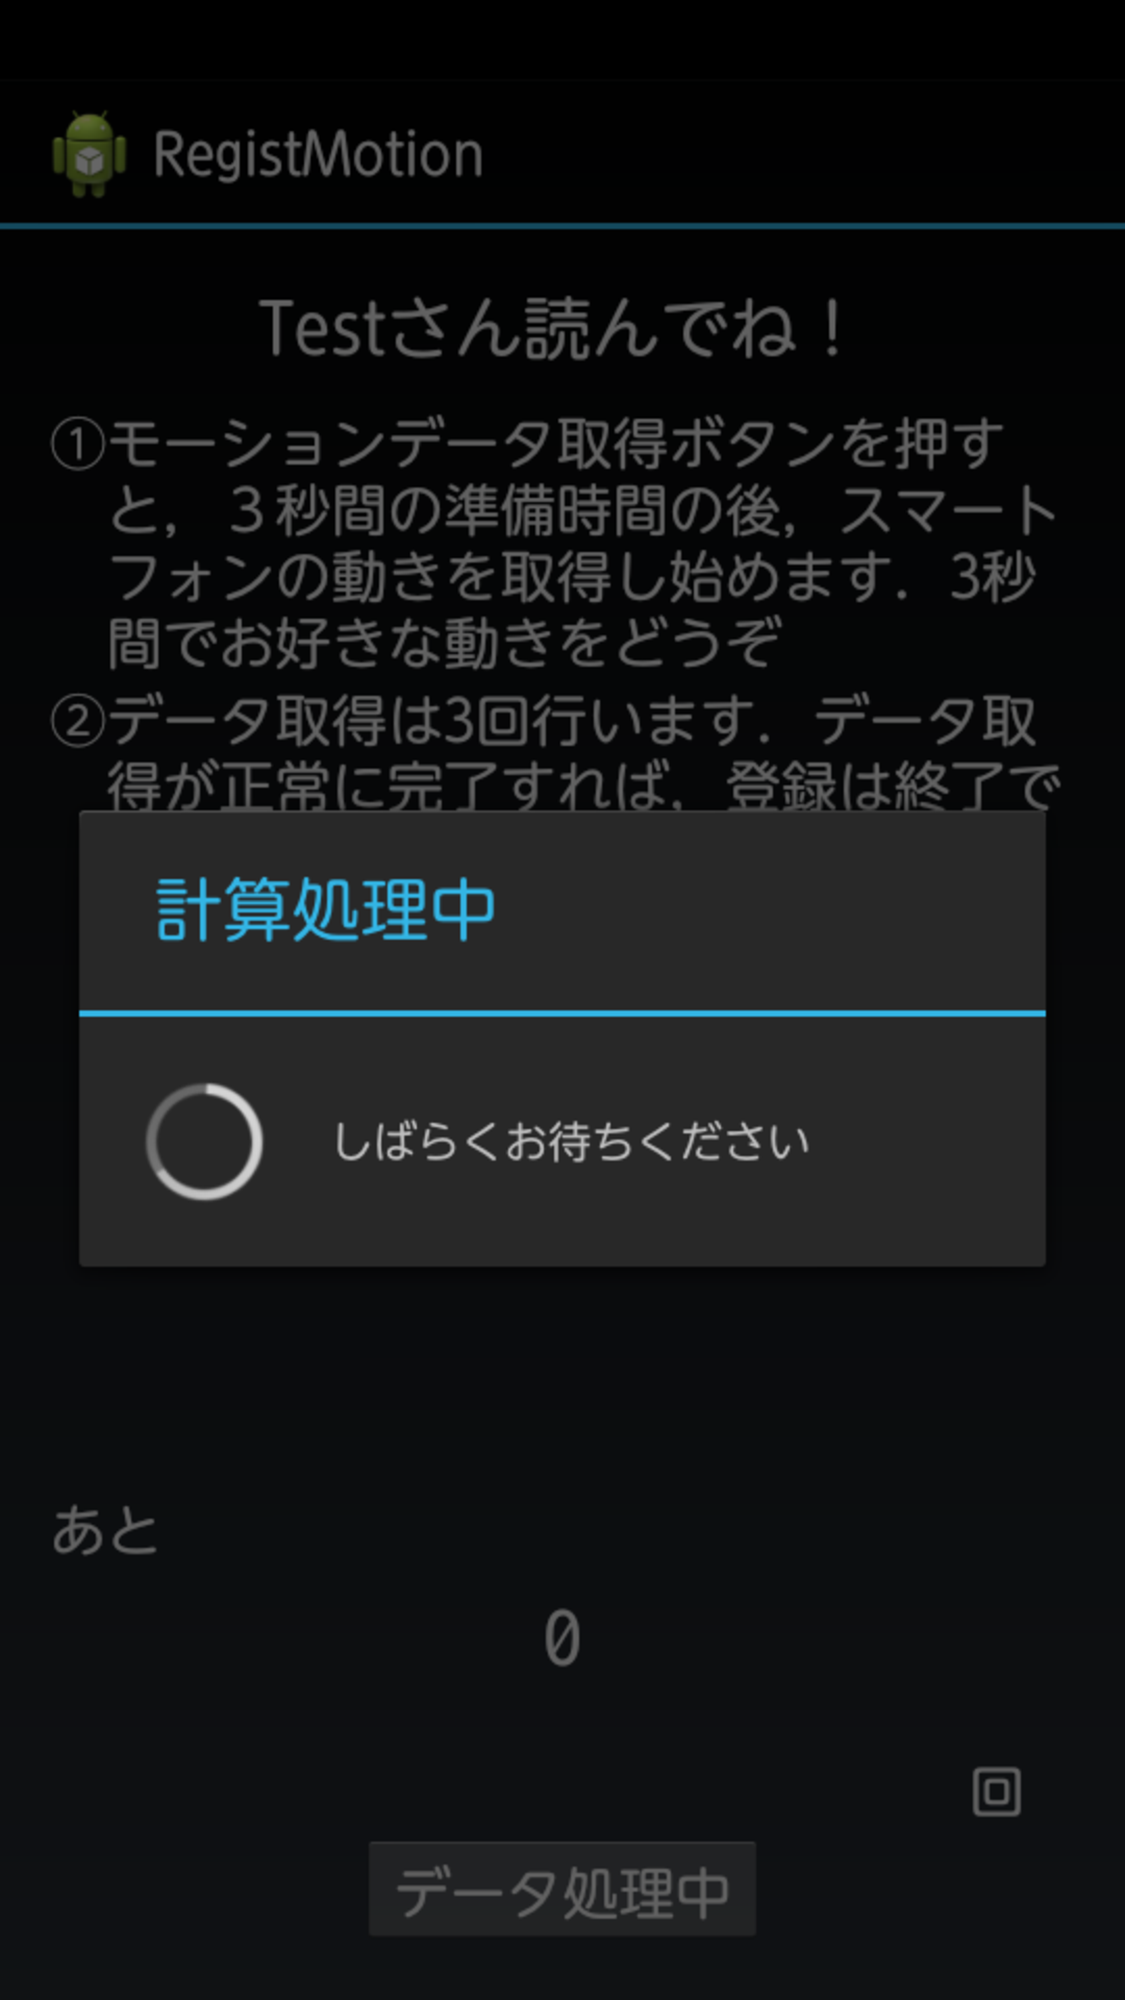
\includegraphics[width=5cm, bb=0 0 540 960]{RegProgress.pdf}
                \end{center}
                \caption{処理待ちダイアログ}
                \label{regProgress}
            \end{minipage}
            \begin{minipage}{0.33\hsize}
                \begin{center}
                    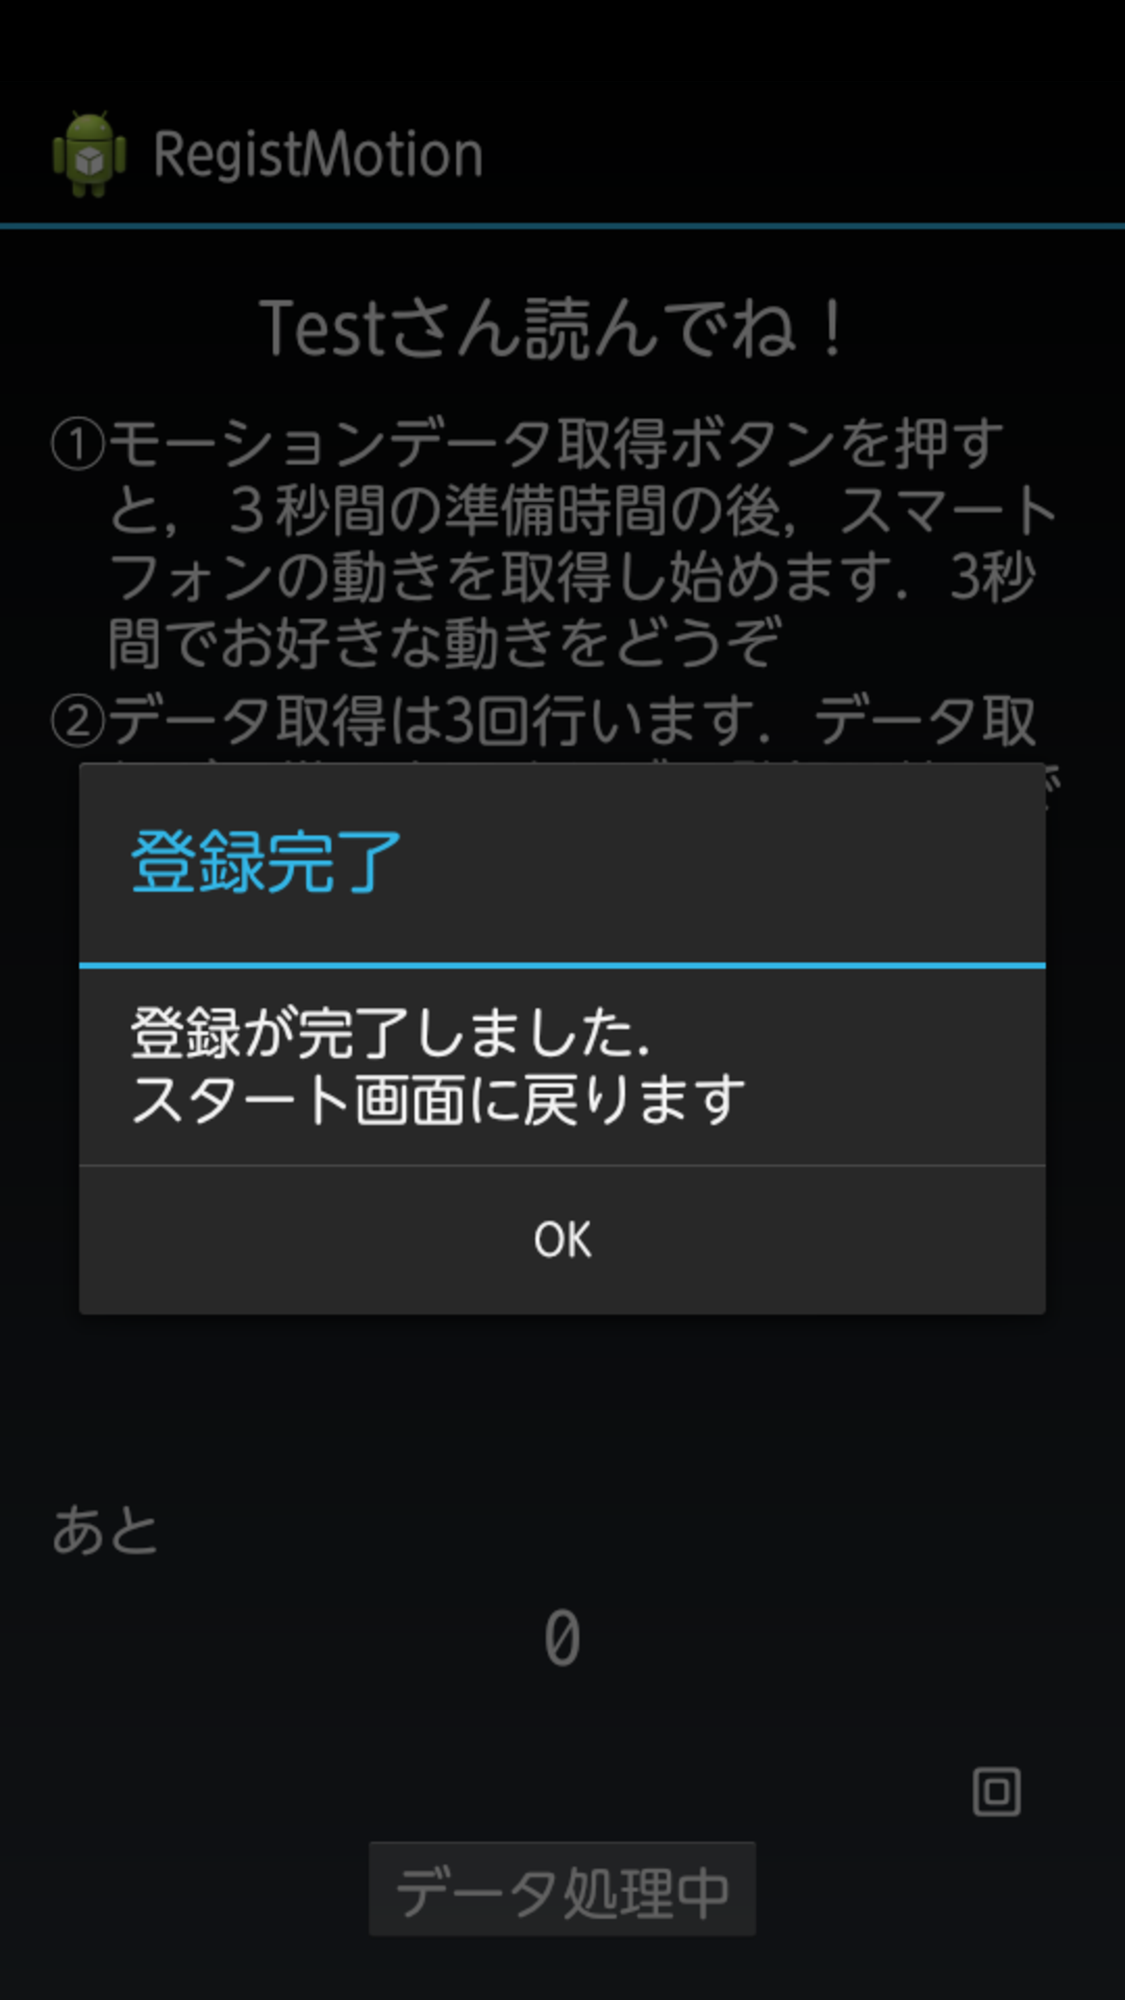
\includegraphics[width=5cm, bb=0 0 540 960]{RegSuccess.pdf}
                \end{center}
                \caption{登録完了ダイアログ}
                \label{regSuccess}
            \end{minipage}
            \begin{minipage}{0.33\hsize}
                \begin{center}
                    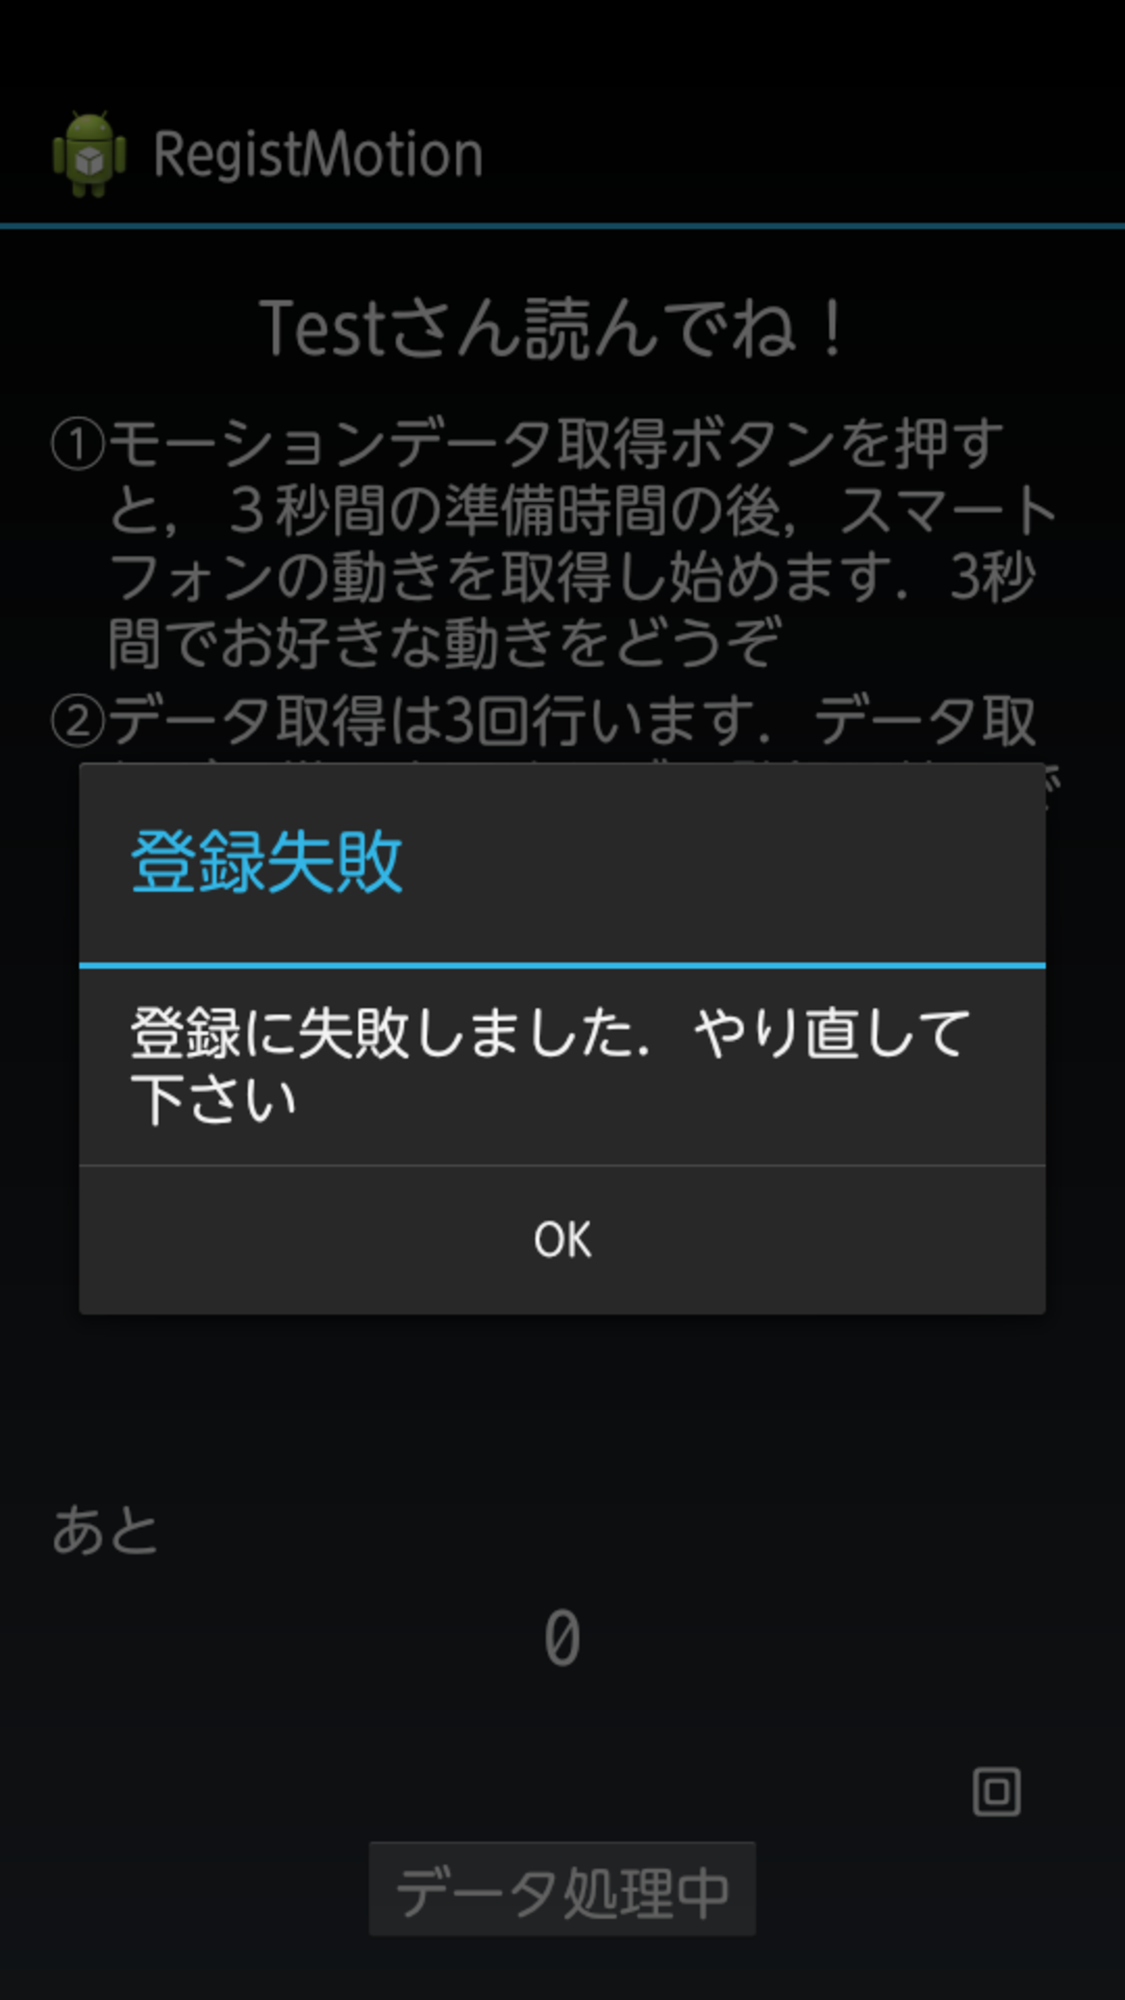
\includegraphics[width=5cm, bb=0 0 540 960]{RegFail.pdf}
                \end{center}
                \caption{登録失敗ダイアログ}
                \label{regFail}
            \end{minipage}
        \end{figure}

	    \subsection{認証試験モード}
        認証試験モードでは,まず図\ref{authNameInput}の画面で新規登録モードであらかじめ登録されたユーザ名を入力させる.
        指定されたユーザ名で既にモーションの登録がなされていることが確認できた場合にのみ,図\ref{auth}の画面で個人認証を行わせる.
        モーションの登録がなされていなかった場合,図\ref{authNameInputError}のようなダイアログを表示する.
        指定されたユーザ名で既にモーションの登録がなされているかを確認するコードをソースコード\ref{authCheckInputNameSource}に示す.

        \begin{figure}[htbp]
            \begin{minipage}{0.33\hsize}
                \begin{center}
                    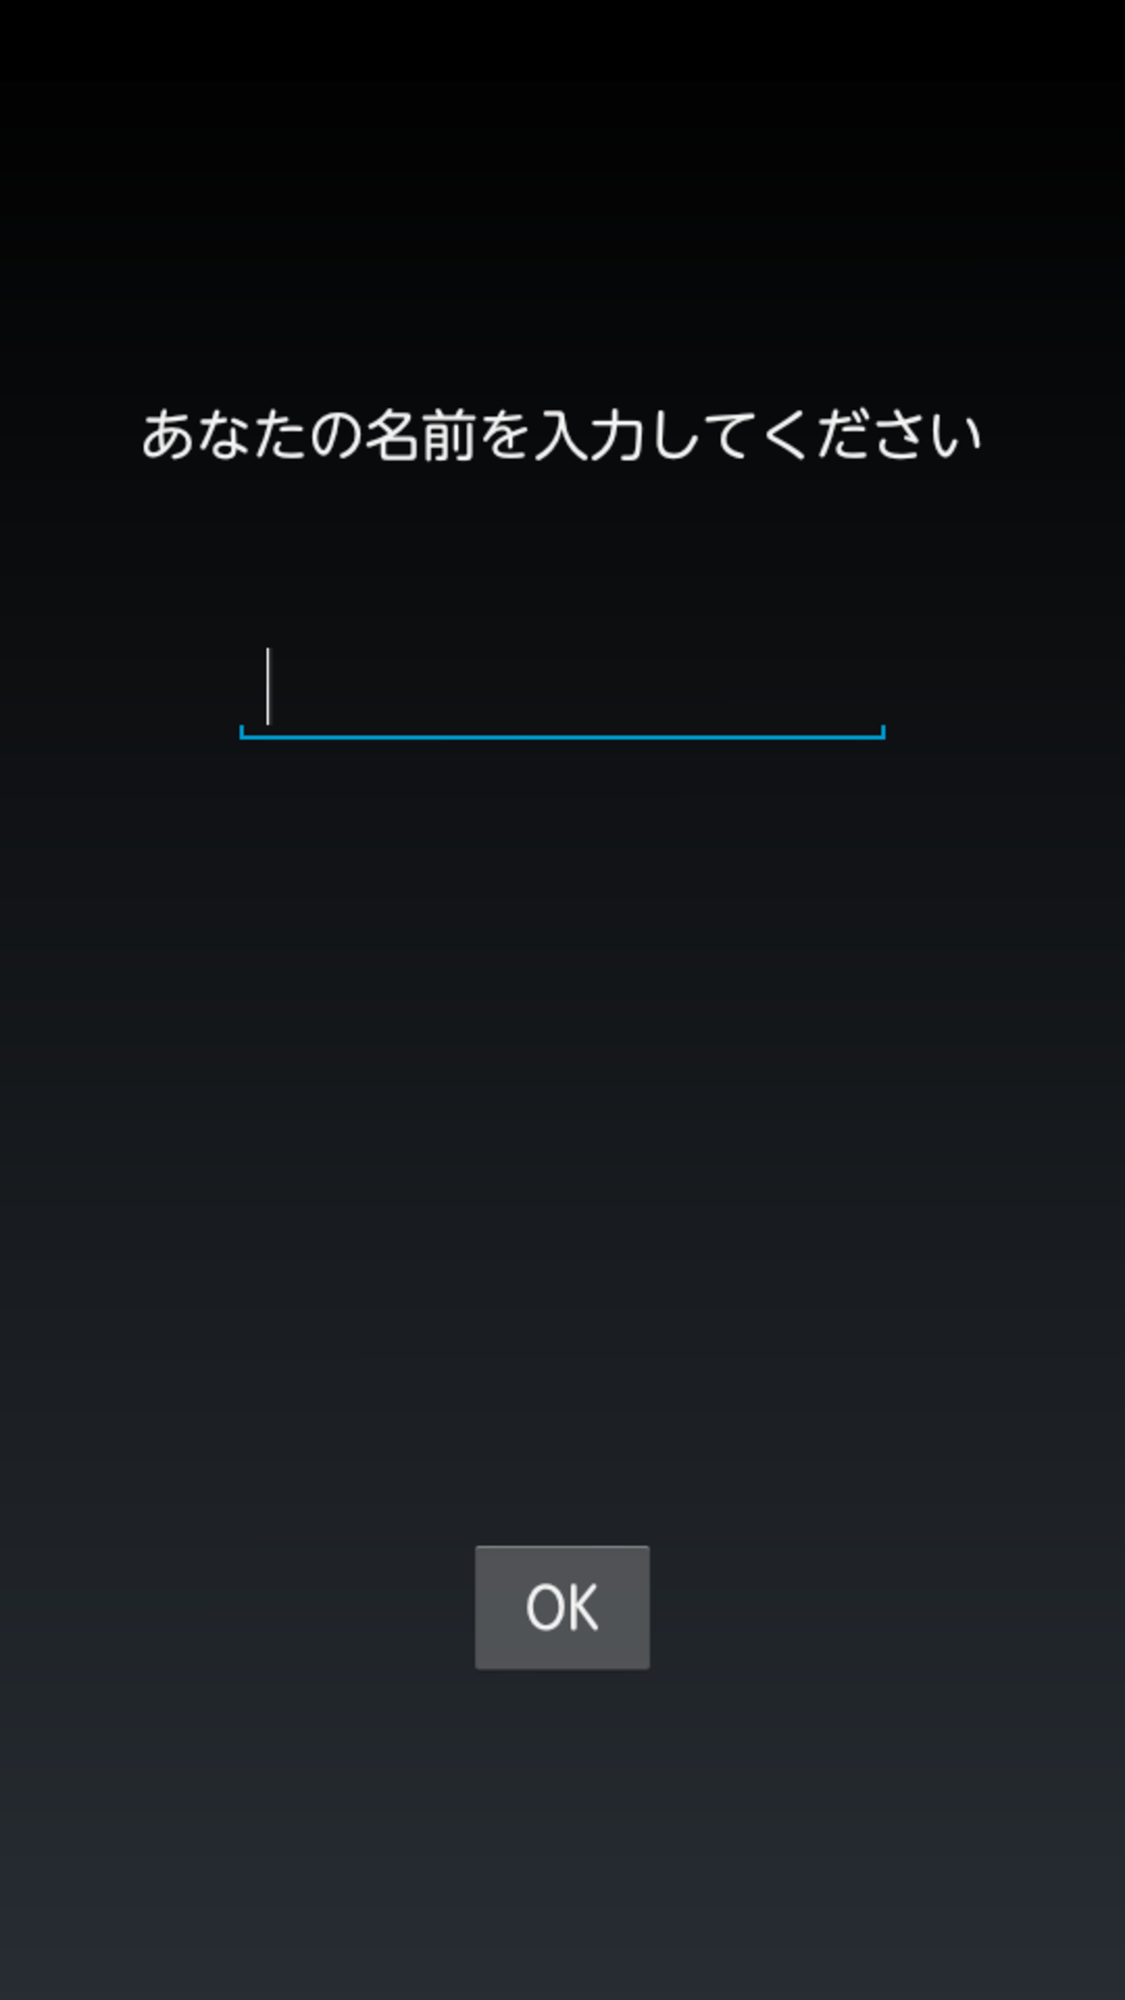
\includegraphics[width=5cm, bb=0 0 540 960]{NameInput.pdf}
                \end{center}
                \caption{ユーザ名入力画面}
                \label{authNameInput}
            \end{minipage}
            \begin{minipage}{0.33\hsize}
                \begin{center}
                    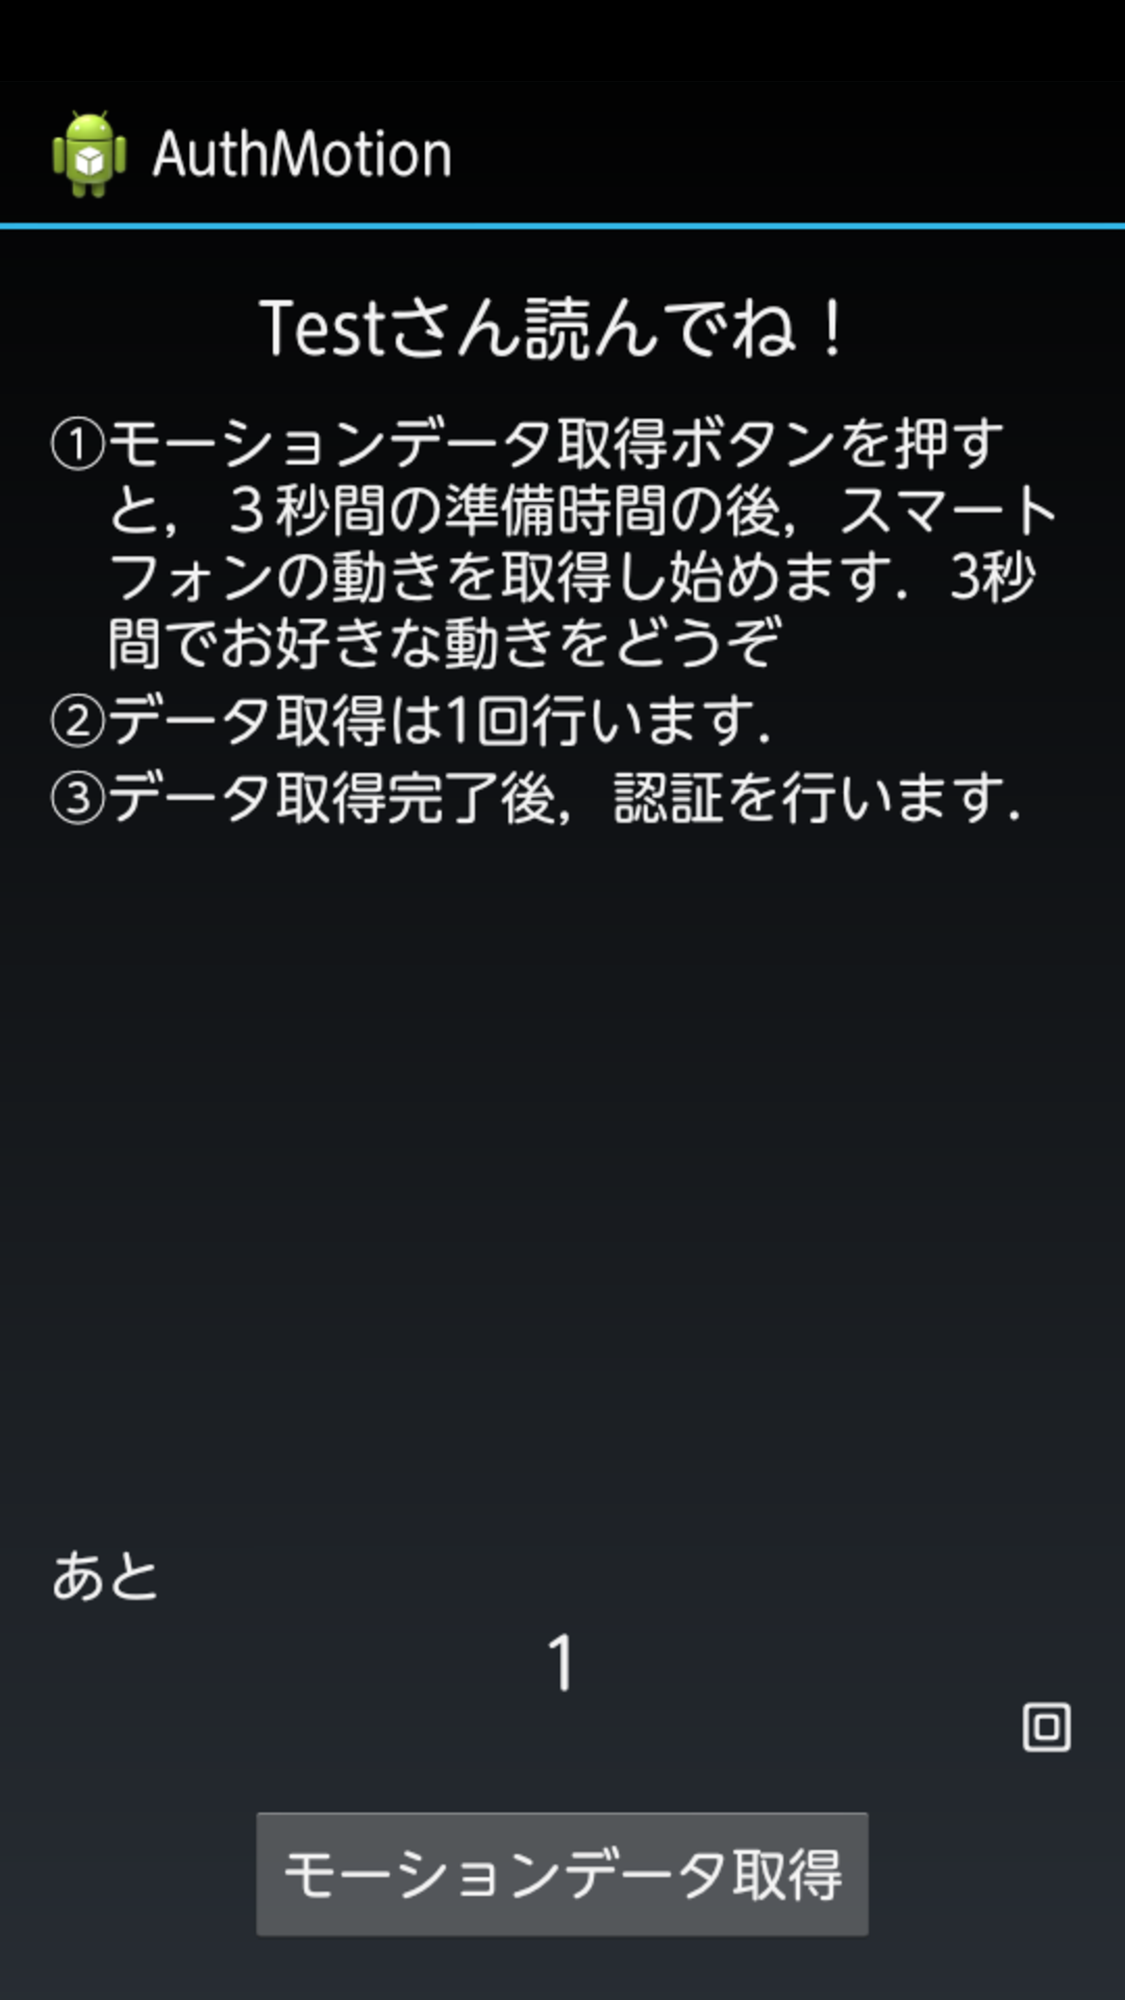
\includegraphics[width=5cm, bb=0 0 540 960]{Auth.pdf}
                \end{center}
                \caption{認証試験画面}
                \label{auth}
            \end{minipage}
            \begin{minipage}{0.33\hsize}
                \begin{center}
                    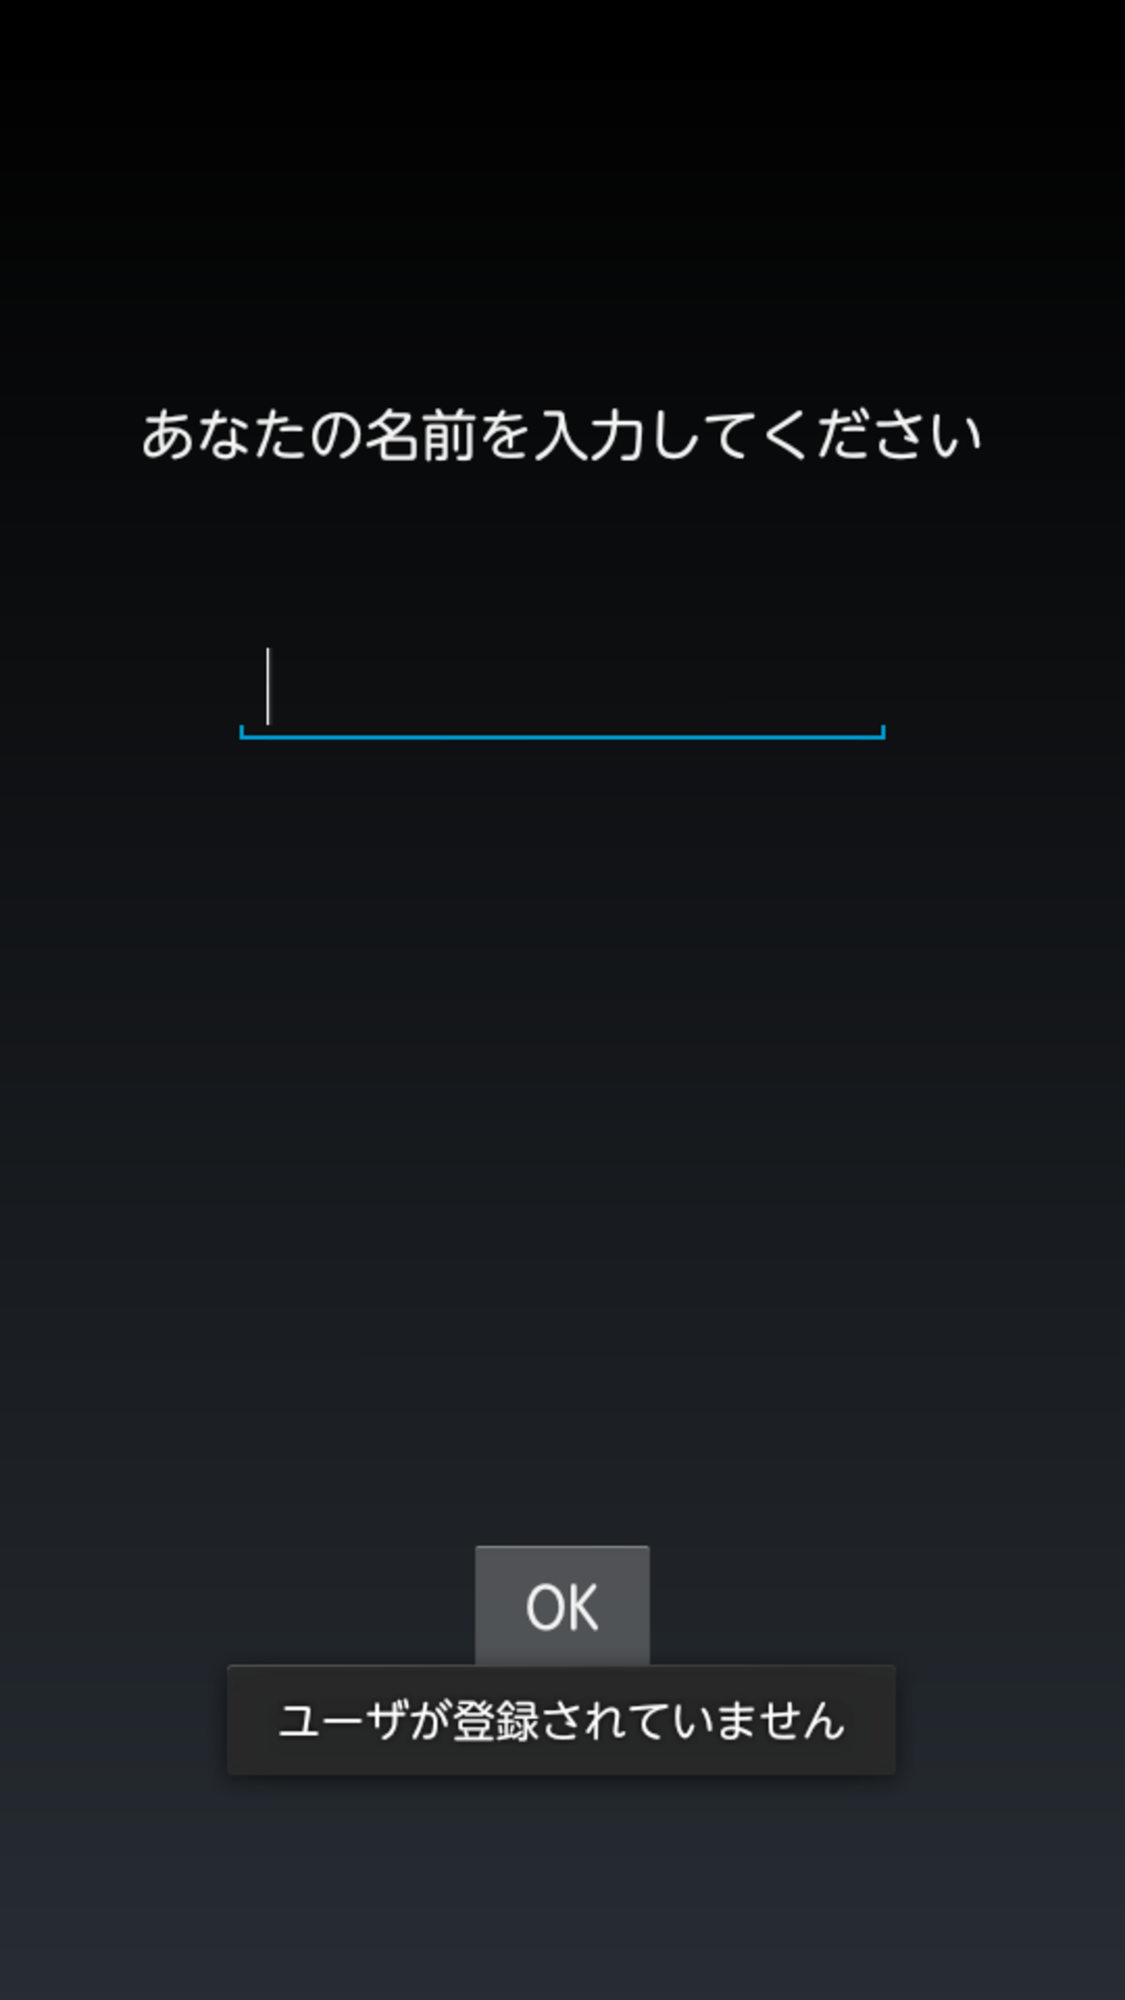
\includegraphics[width=5cm, bb=0 0 540 960]{AuthNameInputError.pdf}
                \end{center}
                \caption{エラー通知}
                \label{authNameInputError}
            \end{minipage}
        \end{figure}

        \newpage
        \lstinputlisting[caption=ユーザ確認, label=authCheckInputNameSource]
        {Code\slash authCheckInputName}

        認証試験モードでは新規登録モードと異なり,1回分のみのモーションデータ取得を行わせる.
        モーションデータの取得後,新規登録モードにおいて登録されたデータに増幅処理が施されていれば,取得したデータに対しても増幅処理を行う.
        そして,フーリエ変換を用いたローパスフィルタ処理を行い,新規登録モードにおいて登録されたデータとの相関係数を算出し個人認証を行う.
        個人認証に成功すれば,図\ref{authSuccess}のような認証成功ダイアログを表示する.
        このダイアログのOKボタンを押すことで,起動画面へと移動する.
        個人認証に失敗すれば,図\ref{authFail}のような認証失敗ダイアログを表示する.
        このダイアログのOKボタンを押すことでプログラム内部のモーションデータ取得カウンタが初期化され,再度個人認証を行えるようにする.

        \begin{figure}[htbp]
            \begin{minipage}{0.5\hsize}
                \begin{center}
                    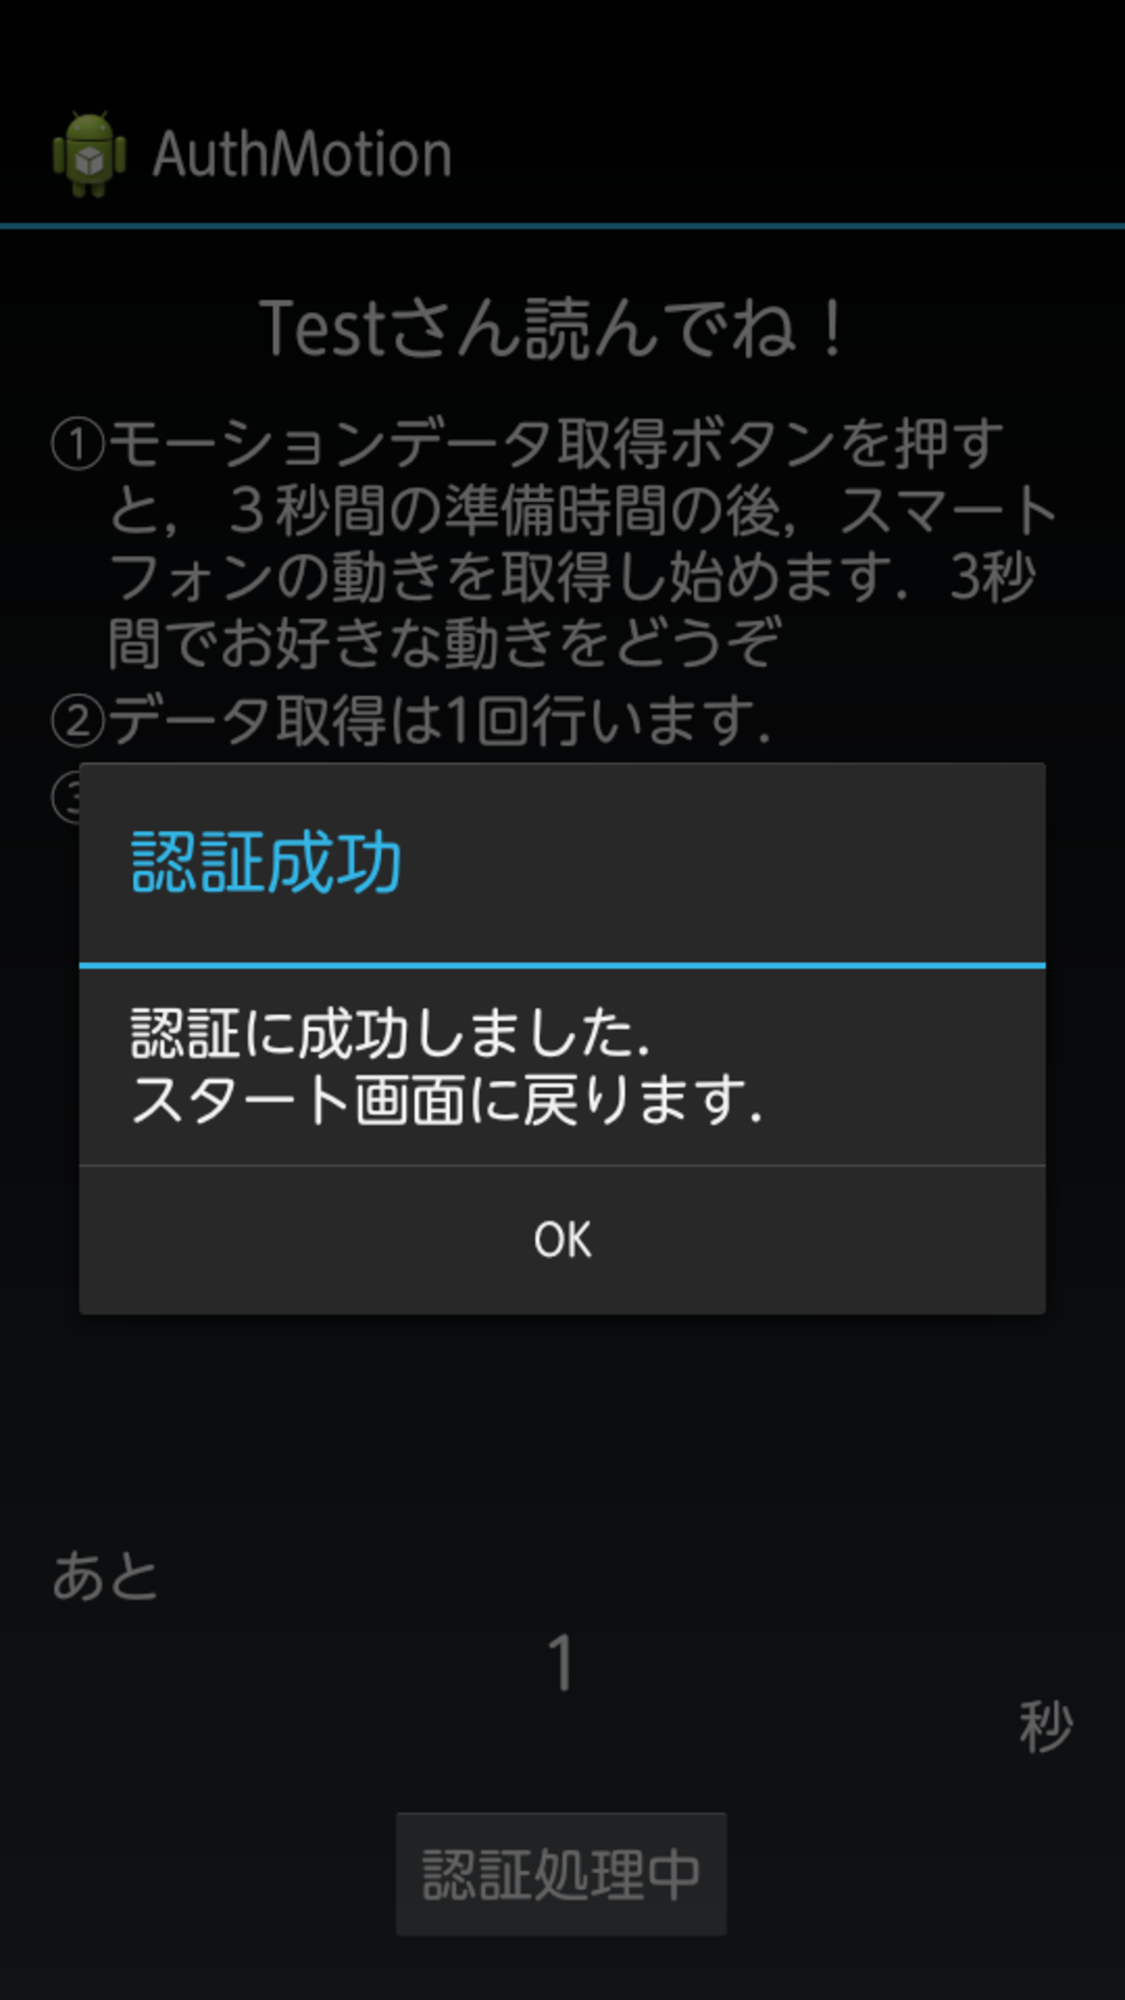
\includegraphics[width=5cm, bb=0 0 540 960]{AuthSuccess.pdf}
                \end{center}
                \caption{認証成功ダイアログ}
                \label{authSuccess}
            \end{minipage}
            \begin{minipage}{0.5\hsize}
                \begin{center}
                    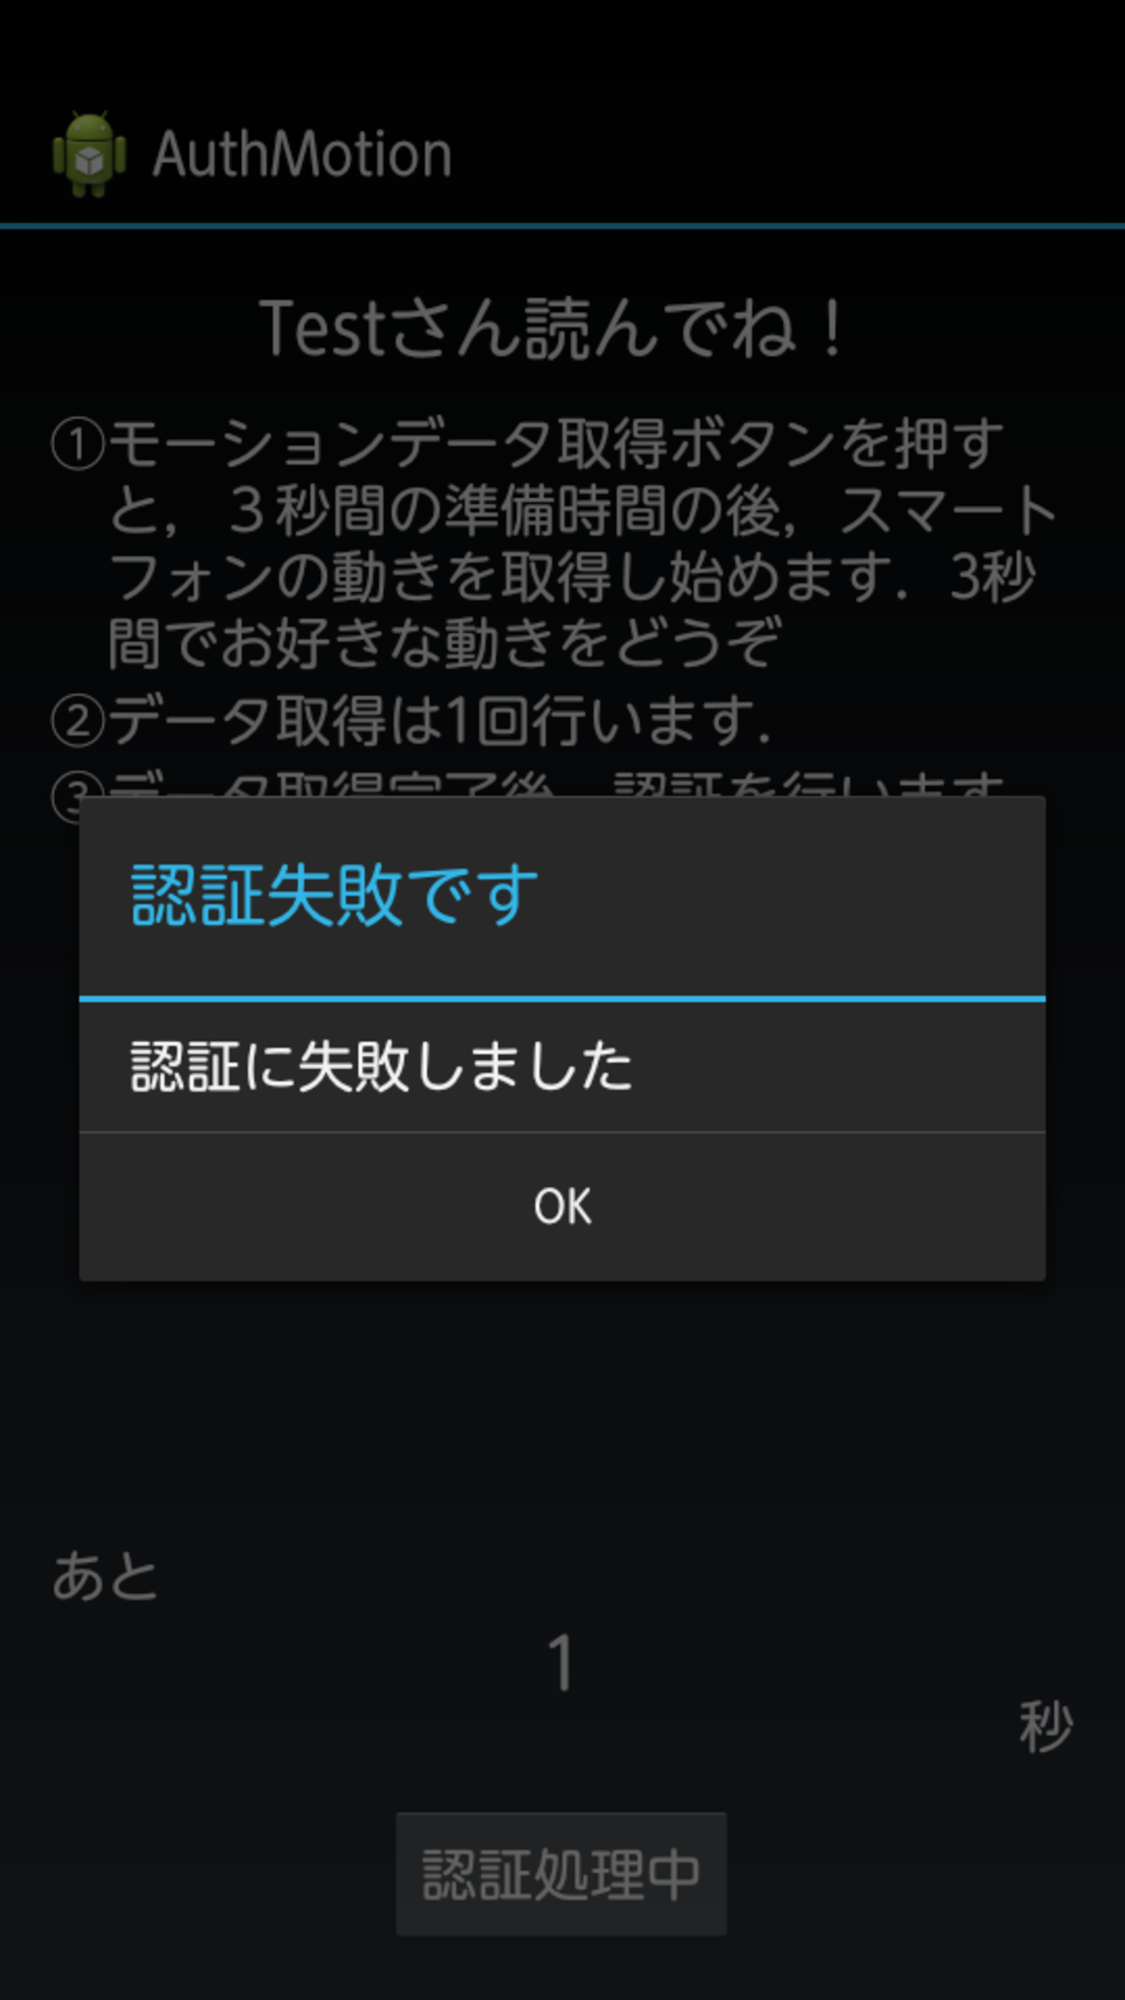
\includegraphics[width=5cm, bb=0 0 540 960]{AuthFail.pdf}
                \end{center}
                \caption{認証失敗ダイアログ}
                \label{authFail}
            \end{minipage}
        \end{figure}

	    \subsection{データ閲覧モード}
	    データ閲覧モードでは,新規登録モードにおいて登録されたユーザ名を一覧で見ることが出来る.
        また,その中からユーザ名を選択するとそのユーザが登録したモーションデータを見ることが出来る.
        このモードを選択すると,まず図\ref{userList}のようなユーザ名の一覧が表示される.
        ここでデータを閲覧したいユーザ名を選択することで,図\ref{dataList}のようなモーションデータ一覧が表示される.

        \begin{figure}[htbp]
            \begin{minipage}{0.5\hsize}
                \begin{center}
                    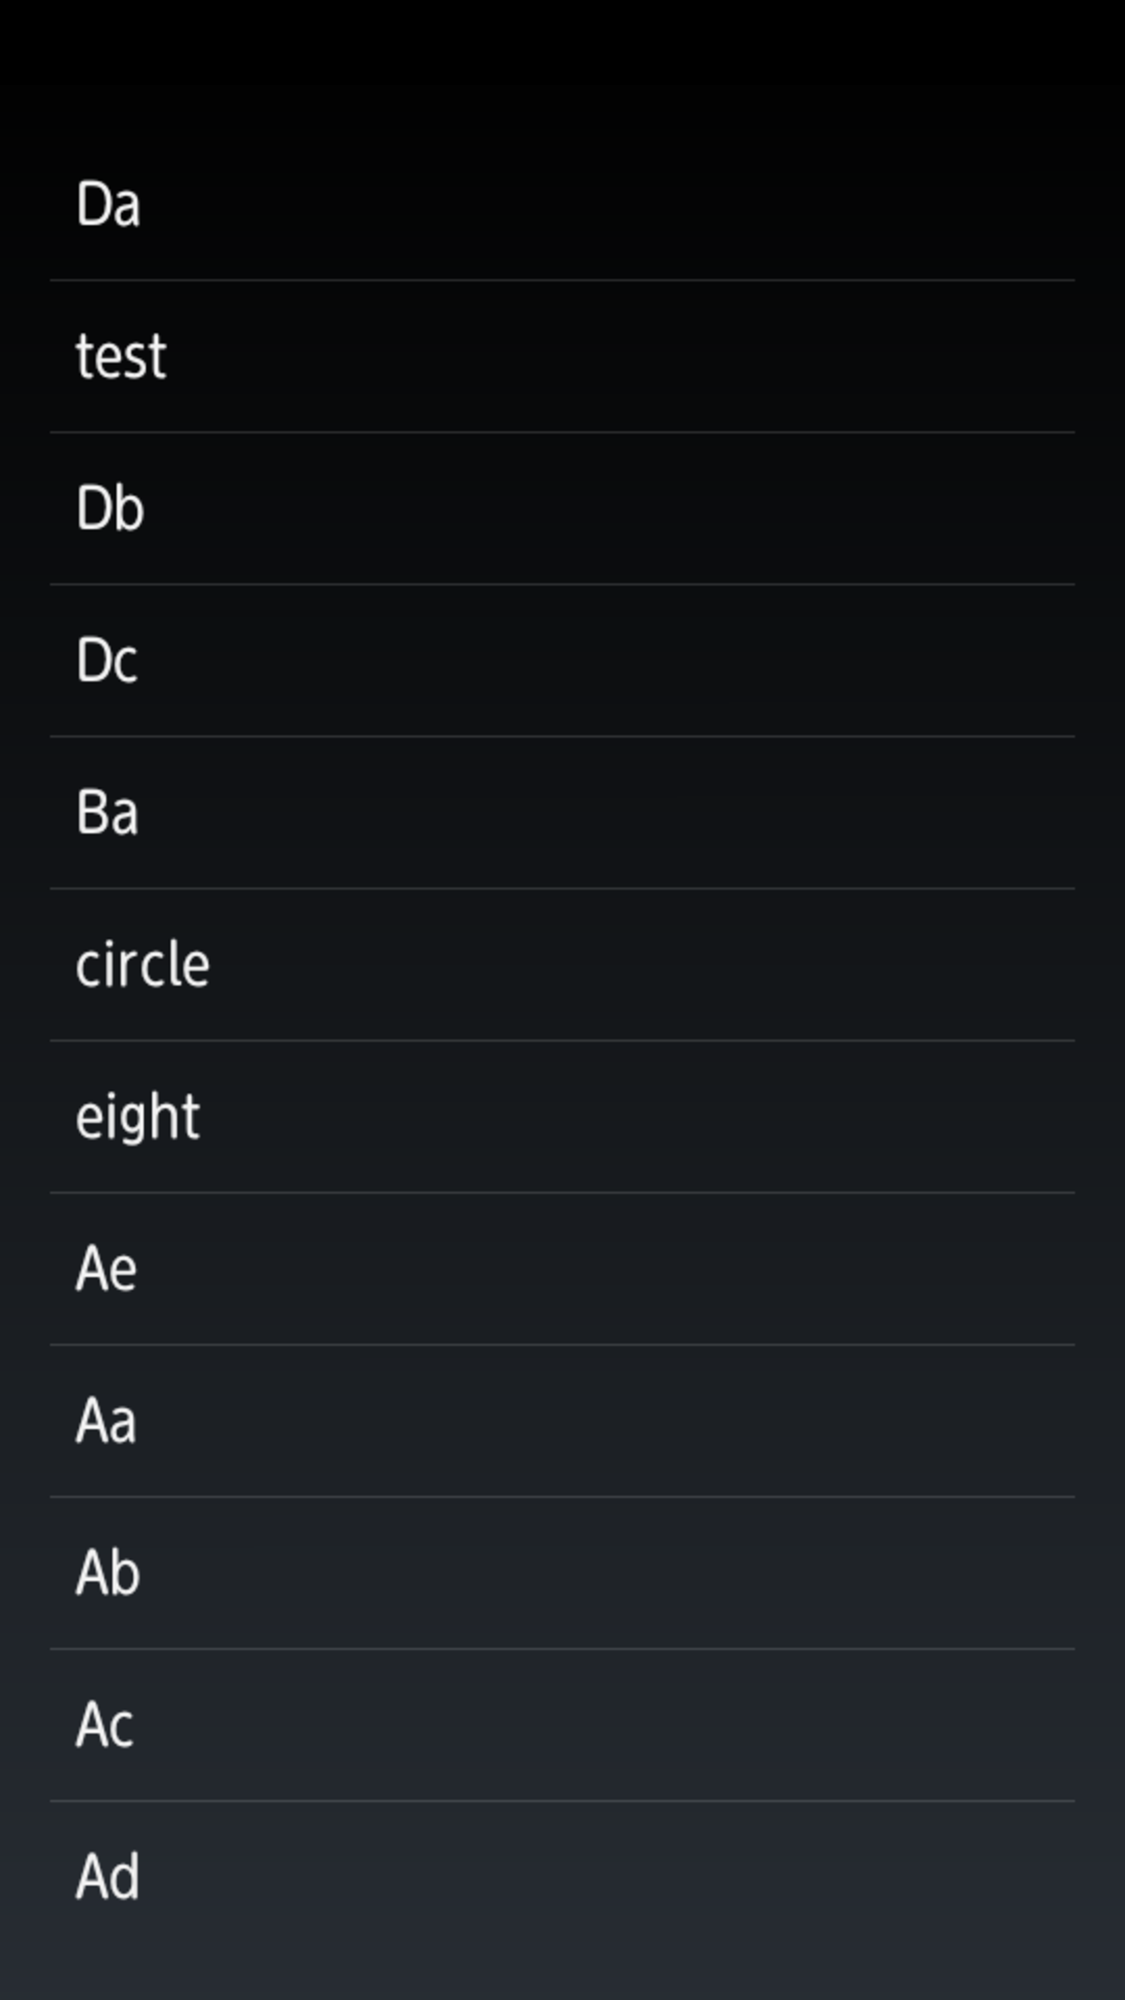
\includegraphics[width=5cm, bb=0 0 540 960]{UserList.pdf}
                \end{center}
                \caption{ユーザ名一覧画面}
                \label{userList}
            \end{minipage}
            \begin{minipage}{0.5\hsize}
                \begin{center}
                    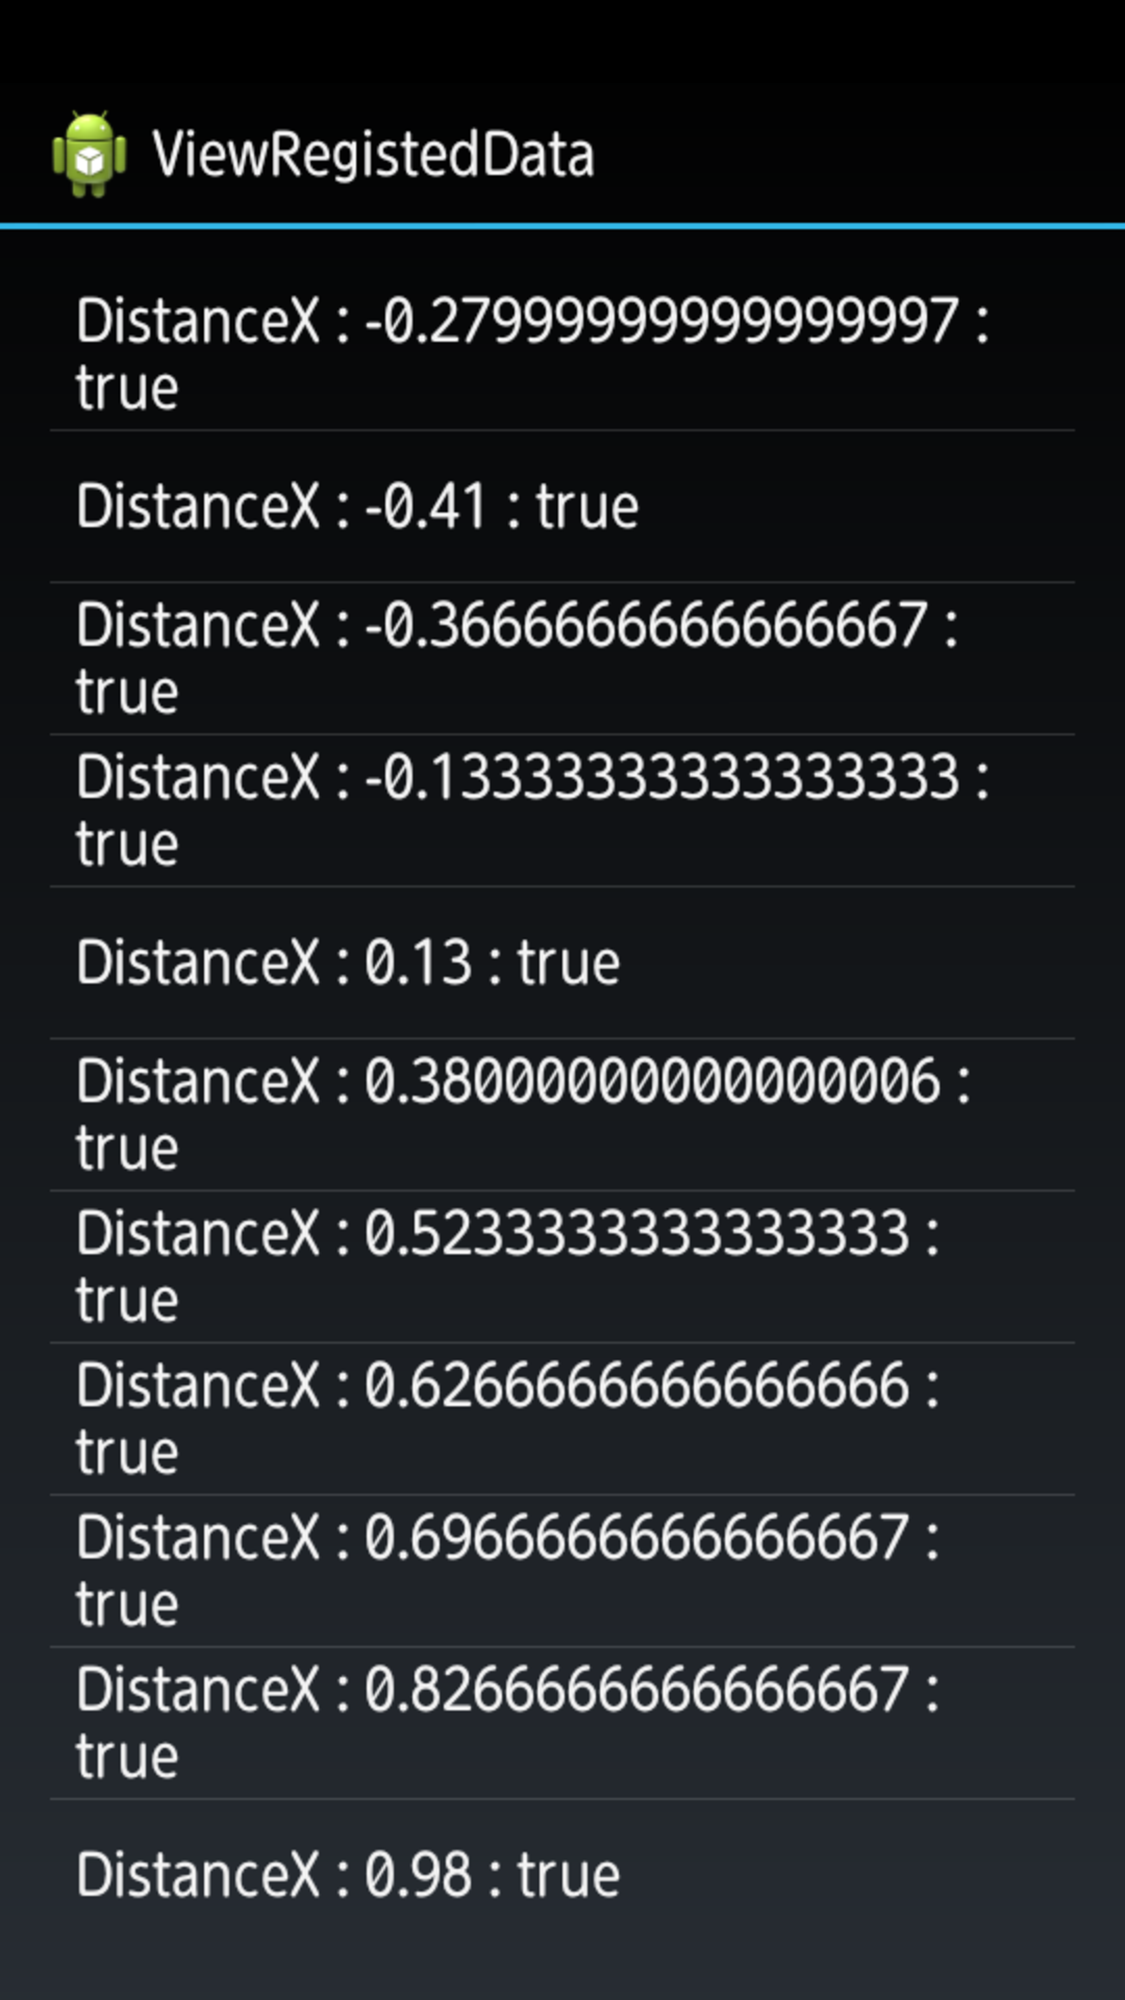
\includegraphics[width=5cm, bb=0 0 540 960]{DataList.pdf}
                \end{center}
                \caption{モーションデータ一覧画面}
                \label{dataList}
            \end{minipage}
        \end{figure}

    \section{先行研究からの改善点}
    先行研究において指摘されていた,手首のスナップを用いるような比較的動きの小さなモーションにおいて,認証率が低く出てしまうという課題を解決するために導入した機能をここに挙げる.

        \subsection{モーションデータの増幅機能}
        手首を中心とするような動きの小さいモーションにおける個人認証成功率を向上させるために,モーションデータの増幅機能を実装した.
        これにより,比較的動きの小さなモーションであってもデータを増幅して用いることができ,比較的動きの大きなモーションと比べて遜色なく用いることが出来るようになった.
        この処理をソースコード\ref{amplifierSource}に示す.

        \lstinputlisting[caption=モーションデータ増幅機能, label=amplifierSource]
        {Code\slash amplifier}

        この増幅機能は,事前にデータの最大値と最小値の差を取り,得られた値があらかじめ設定された閾値を下回った場合にのみ機能するようにしている.
        この処理をソースコード\ref{dataRangeCheckSource}に示す.

        \lstinputlisting[caption=データレンジチェック, label=dataRangeCheckSource]
        {Code\slash dataRangeCheck}

        データをどれだけ増幅させるかを決める値やデータの最大値と最小値の差がどれだけあれば増幅を行うかを決める閾値に関しては,新規登録モードにおいてメニューキーを押すことで表示される図\ref{regMenu}のようなメニュー内の増幅器設定を選択することで表示される,図\ref{amplifierSettings}のような設定ダイアログより変更することが出来る.

    \begin{figure}[htbp]
        \begin{minipage}{0.5\hsize}
            \begin{center}
                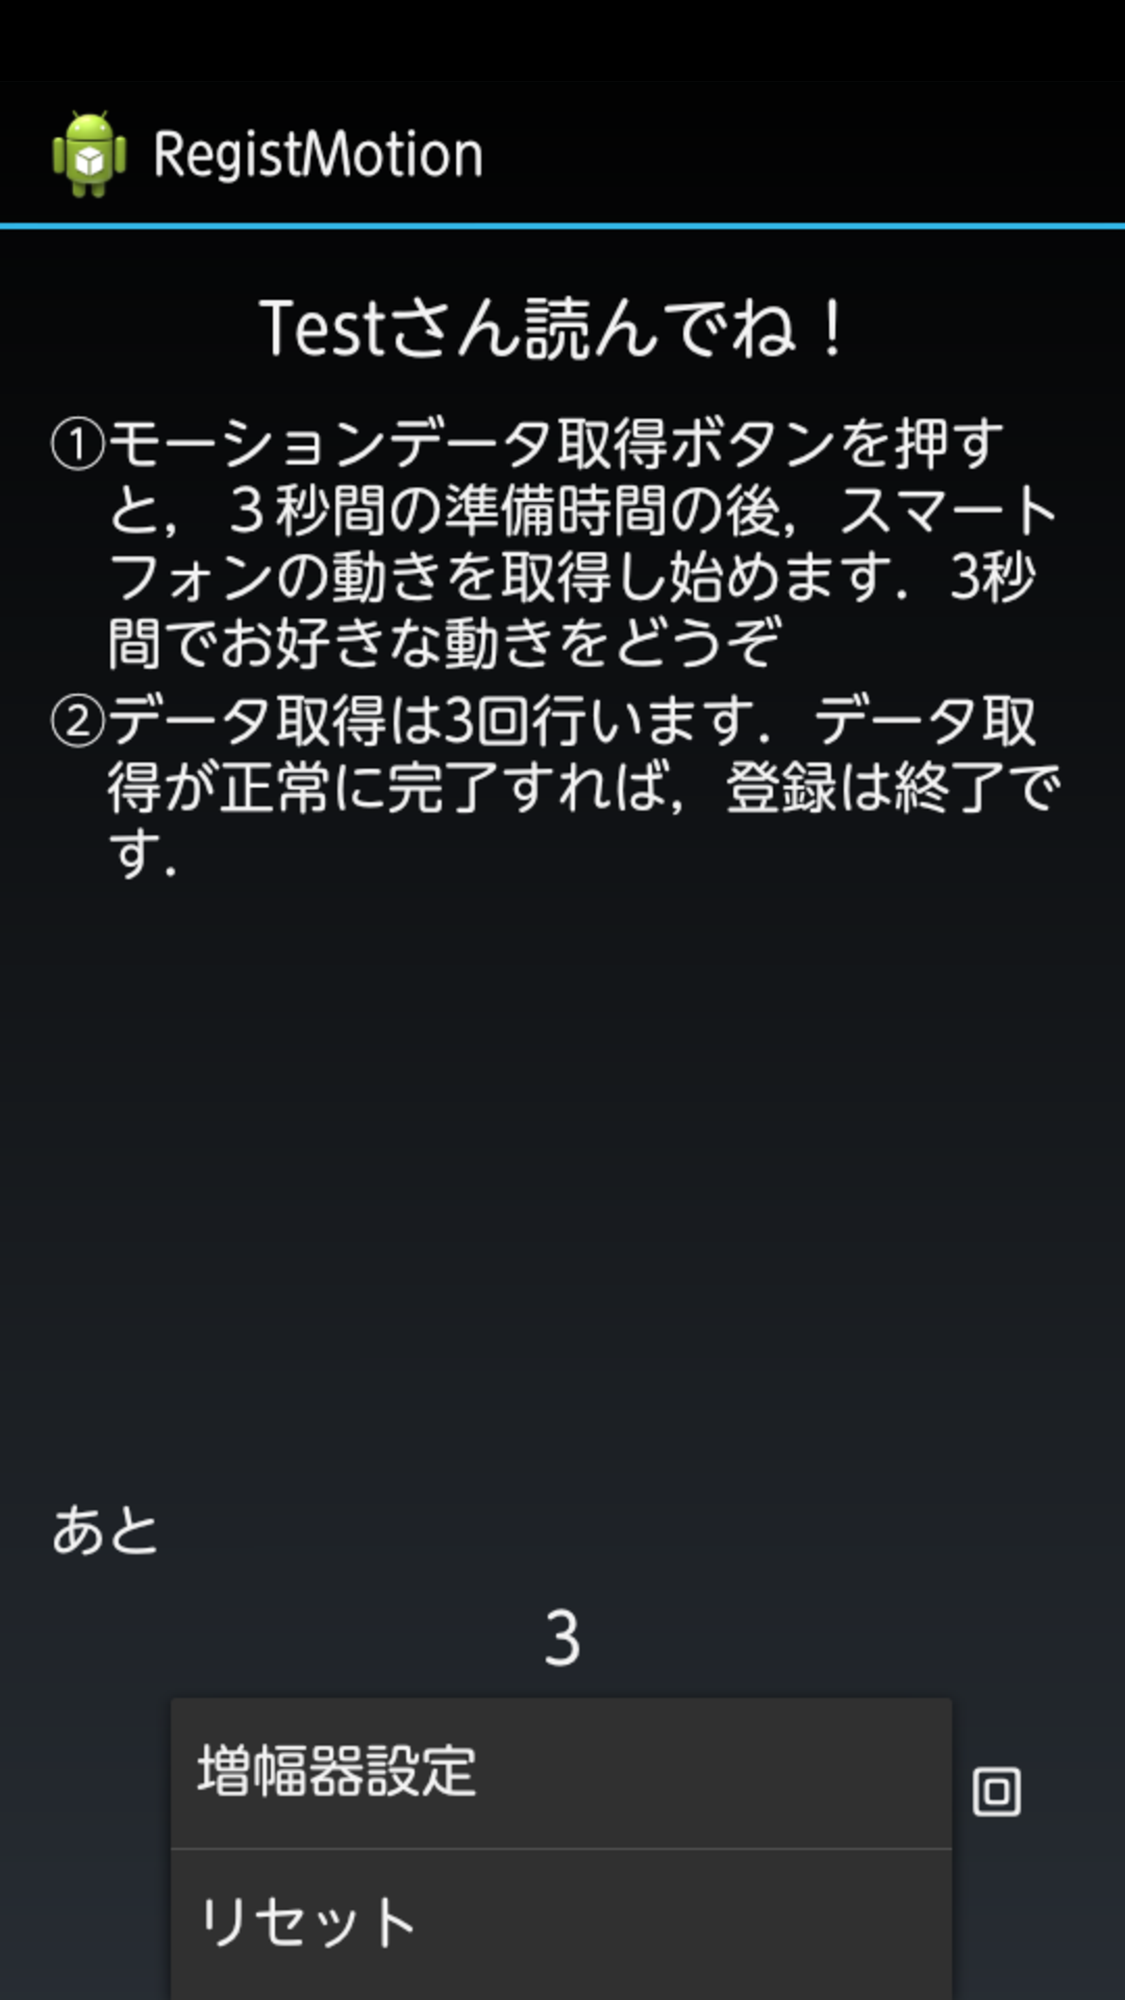
\includegraphics[width=5cm, bb=0 0 540 960]{RegMenu.pdf}
            \end{center}
            \caption{新規登録モードメニュー画面}
            \label{regMenu}
        \end{minipage}
        \begin{minipage}{0.5\hsize}
            \begin{center}
                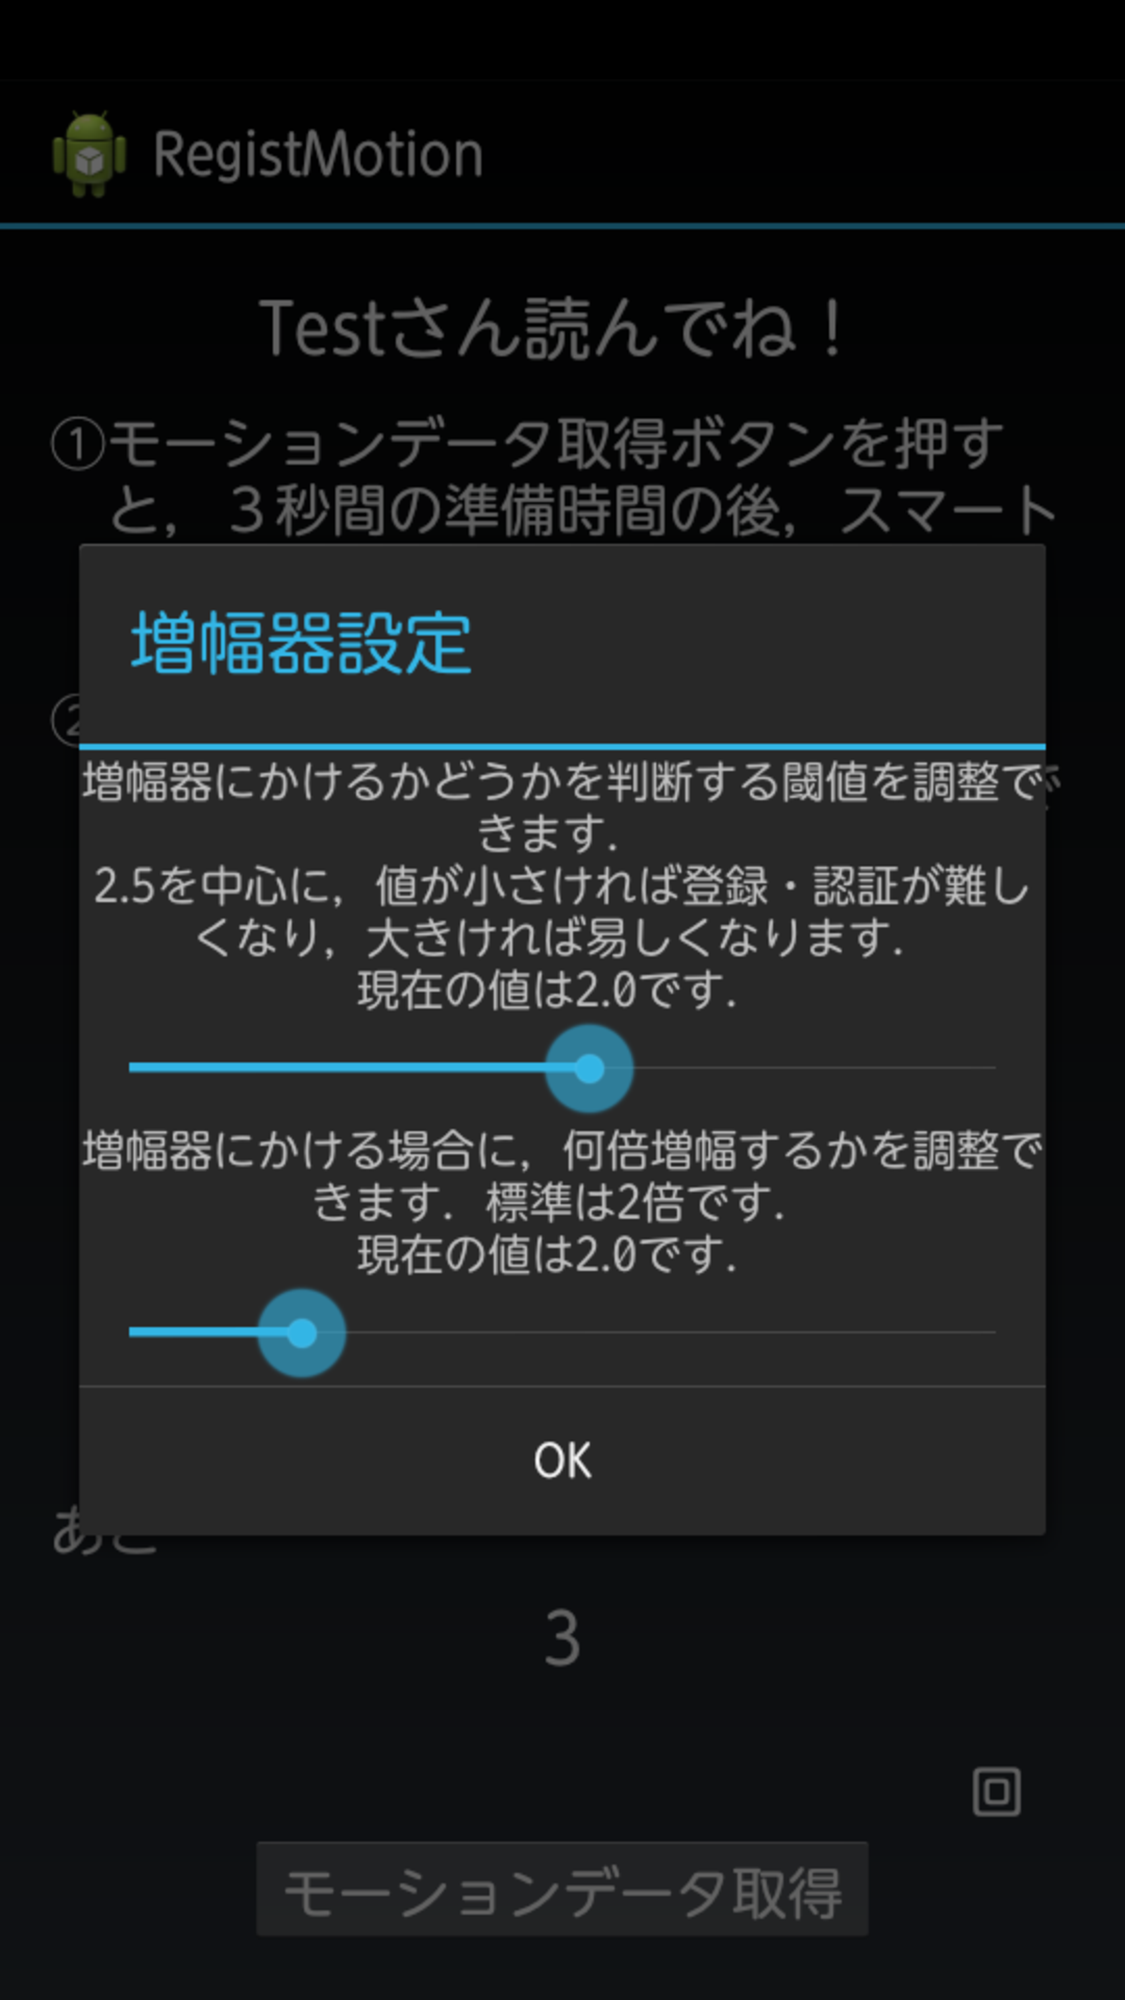
\includegraphics[width=5cm, bb=0 0 540 960]{AmplifierSettings.pdf}
            \end{center}
            \caption{増幅器設定ダイアログ}
            \label{amplifierSettings}
        \end{minipage}
    \end{figure}

        増幅器にかける前のデータをグラフ化したものを図\ref{beforeAmpDataGraph}に,かけた後のデータをグラフ化したものを図\ref{afterAmpDataGraph}に示す.
        % Data : BeforeAMP and AfterAMP

        \begin{figure}[htbp]
            \begin{minipage}{0.5\hsize}
                \begin{center}
                    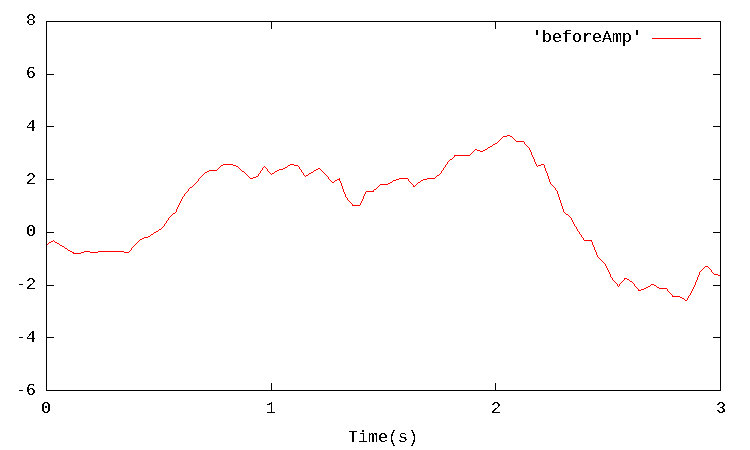
\includegraphics[width=8cm, bb=0 0 360 216]{beforeAmpGraph.pdf}
                \end{center}
                \caption{増幅前のデータ}
                \label{beforeAmpDataGraph}
            \end{minipage}
            \begin{minipage}{0.5\hsize}
                \begin{center}
                    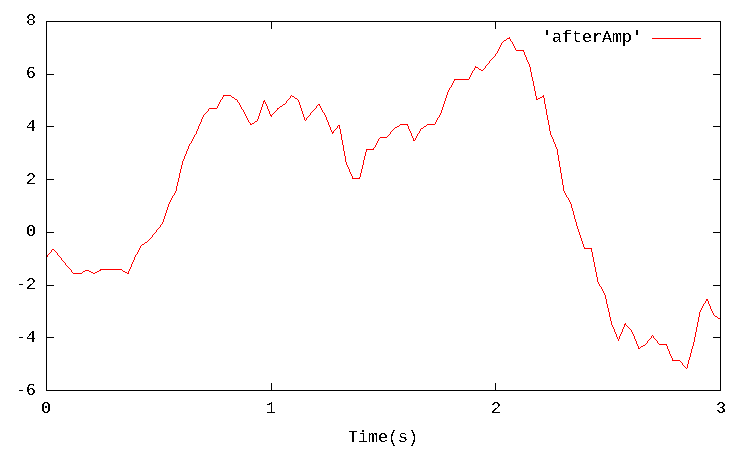
\includegraphics[width=8cm, bb=0 0 360 216]{afterAmpGraph.pdf}
                \end{center}
                \caption{増幅後のデータ}
                \label{afterAmpDataGraph}
            \end{minipage}
        \end{figure}

        \subsection{フーリエ変換を用いたローパスフィルタ}
        モーションデータを取得している際の細かな手の震えなどによるデータに対する影響を取り除き,モーションデータとしての純度を高めるために,フーリエ変換を用いたローパスフィルタ処理を行っている.

        フーリエ変換を用いて時間軸で表されるモーションデータを周波数領域に変換することで,モーション中の細かな手の震えなどのデータが高周波成分として現れる.
        そしてこの高周波成分を取り除いた上で元の時間軸のデータに戻すローパスフィルタ処理を行うことで,細かな手の震えなどによるデータに対する影響を取り除いている.
        フーリエ変換を実装する際には,CERNのColt Project\cite{coltproj}で開発されたJavaによる科学技術計算用ライブラリであるColt\cite{colt}をマルチスレッド化したParallel Colt\cite{parallelcolt}に含まれている,JTransforms\cite{jtransforms}を用いて実装している.
        この処理をソースコード\ref{lowpassSource}に示す.

        % 付録に回す
        \lstinputlisting[caption=ローパスフィルタ処理, label=lowpassSource]
        {Code\slash lowpass}

        ローパスフィルタにかける前のデータをグラフ化したものを図\ref{beforeLowpassDataGraph}に,かけた後のデータをグラフ化したものを図\ref{afterLowpassDataGraph}に示す.

        \begin{figure}[htbp]
            \begin{minipage}{0.5\hsize}
                \begin{center}
                    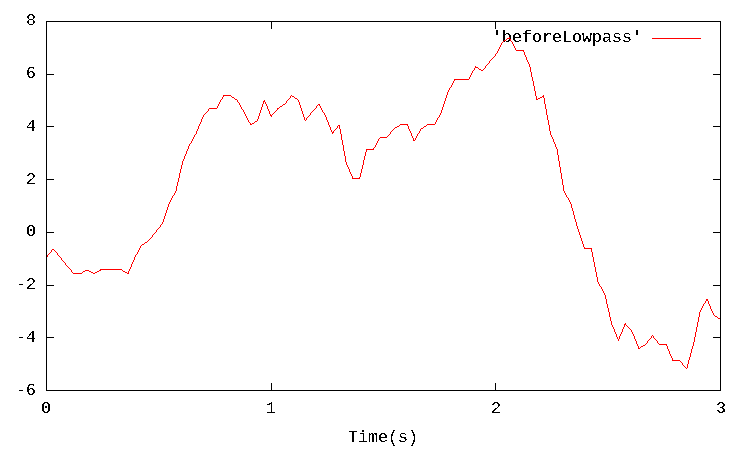
\includegraphics[width=8cm, bb=0 0 360 216]{beforeLowpassGraph.pdf}
                \end{center}
                \caption{ローパスフィルタ前のデータ}
                \label{beforeLowpassDataGraph}
            \end{minipage}
            \begin{minipage}{0.5\hsize}
                \begin{center}
                    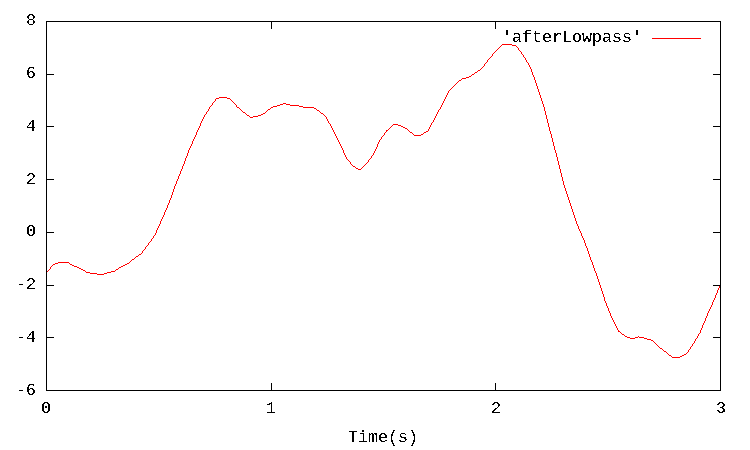
\includegraphics[width=8cm, bb=0 0 360 216]{afterLowpassGraph.pdf}
                \end{center}
                \caption{ローパスフィルタ後のデータ}
                \label{afterLowpassDataGraph}
            \end{minipage}
        \end{figure}

        \subsection{モーション取得時のズレを修正する機能}
        新規登録モードにおいてモーションを登録する際には3回分のモーションデータの入力が必要になるが,この回数ごとにモーションの時間的なズレが生じた場合はデータ登録や認証時に影響を与えてしまう可能性があるため,このズレを修正する処理を3回分のデータ取得後に行うようにしている.

        3回分のデータ取得後,まずはこのデータ間の相関係数を算出し,回数ごとに全く別のモーションが入力されていないかの確認を行う.
        そしてある程度以上の相関が見られるが,それでも相関係数が低く出てしまった場合に,ズレ修正後の相関係数を確認しつつ,データの最大値に合わせるパターン,データの最小値に合わせるパターン,データの中央値に合わせるパターンの最大三つの方法で相関係数の向上を試みる.
        この部分のコードをソースコード\ref{checkDeviationSource}に示す.

        \lstinputlisting[caption=ズレ修正判断部分, label=checkDeviationSource]
        {Code\slash checkDeviation}

        相関係数を算出した結果,ズレ修正が必要であると判断された場合,付録のソースコード\ref{correctDeviationSource}に示したズレ修正アルゴリズムを用いて修正を行う.

        ズレ修正を行う前のデータをグラフ化したものを図\ref{beforeDeviationDataGraph}に,修正を行った後のデータをグラフ化したものを図\ref{afterDeviationDataGraph}に示す.

        % 修正前と修正後の比較グラフ
        \begin{figure}[htbp]
            \begin{minipage}{0.5\hsize}
                \begin{center}
                    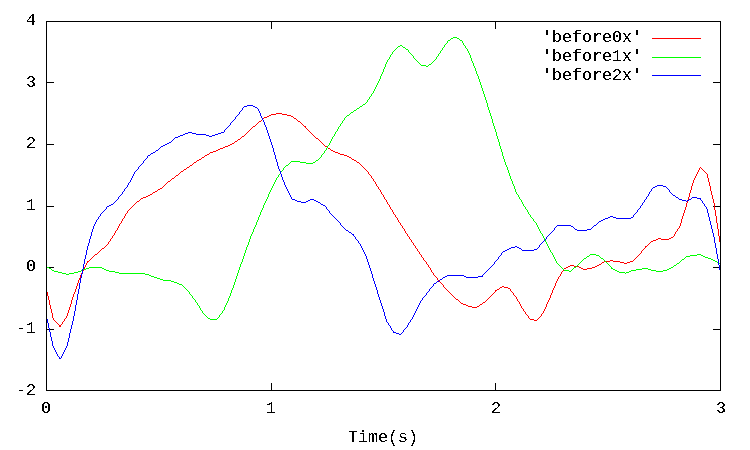
\includegraphics[width=8cm, bb=0 0 360 216]{beforeDeviationGraph.pdf}
                \end{center}
                \caption{ズレ修正前のデータ}
                \label{beforeDeviationDataGraph}
            \end{minipage}
            \begin{minipage}{0.5\hsize}
                \begin{center}
                    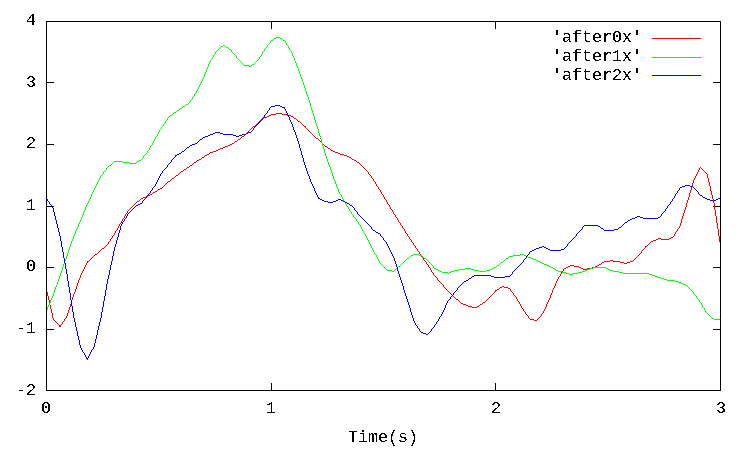
\includegraphics[width=8cm, bb=0 0 360 216]{afterDeviationGraph.pdf}
                \end{center}
                \caption{ズレ修正後のデータ}
                \label{afterDeviationDataGraph}
            \end{minipage}
        \end{figure}

        \subsection{モーション取得時のインターバル及びヴァイブレーション機能}
        新規登録モード及び認証試験モードにおいてモーション取得時の時間経過が把握しやすいように,1秒毎に端末をヴァイブレーションさせる機能を実装した.
        また,データ取得時のインターバルからデータ取得に移る際には通常より長めのヴァイブレーションにすることで,データ取得開始のタイミングを明確に意識できるようにした.

\chapter{実験と考察}
    \textcolor{red}{改めて実験を行った後,おわりにの部分を含めて修正します}
	\section{実験方法}
	今回開発したシステムを用いて,以下に挙げるそれぞれのモーションを新規登録モードにてあらかじめ登録しておき,認証試験モードにて個人認証の成功率を検証する.
    認証はそれぞれのモーションにつき10回ずつ行い,この結果から個人認証の成功率を算出する.

	\section{実験結果}
	\textcolor{red}{実験結果を表を用いて示す}

	\section{考察}
    \textcolor{red}{実験結果に対する考察}

	\section{課題}
	\textcolor{red}{実験結果より生じた課題}

\chapter{おわりに}
\textcolor{red}{実験終了後,記述します.}

\chapter*{謝辞}
本研究のプログラム開発や実験,本論文の執筆にあたり,手厚い指導と様々な助言をしていただいた,関西大学総合情報学部セキュア情報システム研究室の小林孝史准教授に深く感謝いたします.
また,研究テーマの選定をはじめ,日頃から有益なアドバイスを頂いた同研究室の皆様に感謝いたします.

\begin{thebibliography}{9}
    \bibitem{sakamoto}{坂本 翔,ユーザの直感的な入力をとらえるための3軸加速度センサによるジェスチャ認識の研究,2009年度公立はこだて未来大学卒業論文.}
    \bibitem{tozawa}{兎澤星伸,三軸加速度センサ及び三軸ジャイロセンサを用いた認証アプリケーションの開発,2012年度卒業研究.}
    \bibitem{coltproj}{Colt Project,https:\slash \slash dst.lbl.gov\slash ACSSoftware\slash colt\slash ,2014年12月27日確認.}
    \bibitem{colt}{Colt,https:\slash \slash github.com\slash carlsonp\slash Colt,2014年12月27日確認.}
    \bibitem{parallelcolt}{Parallel Colt,https:\slash \slash sites.google.com\slash site\slash piotrwendykier\slash software\slash parallelcolt,2014年12月27日確認.}
    \bibitem{jtransforms}{JTransforms,https:\slash \slash sites.google.com\slash site\slash piotrwendykier\slash software\slash jtransforms,2014年12月27日確認.}
\end{thebibliography}

\appendix

\chapter{ソースコード}
%    \section{ズレ修正の判断部分}
%    \lstinputlisting[label=checkDeviationSource]
%    {Code\slash checkDeviation}

    \section{ズレ修正アルゴリズム}
    \lstinputlisting[label=correctDeviationSource]
    {Code\slash correctDeviation}
\end{document}
